\documentclass[UTF8,11pt]{article}

  % Package for using the full page.
  \usepackage{fullpage}

  % Package for writing algorithms (why do we need this one?).
  \usepackage[linesnumbered,ruled,vlined]{algorithm2e}

  % Package for using colored texts.
  \usepackage[dvipsnames]{xcolor}

  % Pakcage for using multiple optional parameters in new commands.
  \usepackage{xargs}

  % Packages for writing comments and todo notes.
  \usepackage[colorinlistoftodos,prependcaption,textsize=tiny]{todonotes}
  \newcommandx{\unsure}[2][1=]
    {\todo[linecolor=red,backgroundcolor=red!25,
 bordercolor=red,#1]
 {#2}\xspace{}}
  \newcommandx{\change}[2][1=]
    {\todo[linecolor=blue,backgroundcolor=blue!25,
 bordercolor=blue,#1]
 {#2}\xspace{}}
  \newcommandx{\info}[2][1=]
    {\todo[linecolor=OliveGreen,backgroundcolor=OliveGreen!25,
 bordercolor=OliveGreen,#1]
 {#2}}
  \newcommandx{\improvement}[2][1=]
    {\todo[linecolor=Plum,backgroundcolor=Plum!25,bordercolor=Plum,#1]
 {#2}\xspace{}}
  \newcommandx{\thiswillnotshow}[2][1=]
    {\todo[disable,#1]
 {#2}\xspace{}}

  % What are there for?
  % Select what to do with todonotes:
  % \usepackage[disable]{todonotes} % notes not showed
  % \usepackage[draft]  {todonotes} % notes showed

  % Select what to do with command \comment:
  % \newcommand{\comment}[1]
      {}                                    %comment not showed
  \newcommand{\comment}[1]
    {\par {\bfseries \color{blue} #1 \par}} %comment showed

  % ams math packages.
  \usepackage{amsmath, amssymb, amsthm, mathtools,prftree}
  \usepackage{txfonts}

  % Declare a global counter for theorem environments:
  \newcounter{thmcounter}

  % Define new theorem styles and theorem environments.
  \theoremstyle{plain}

  \newtheorem{theorem}    [thmcounter]{Theorem}
  \newtheorem{corollary}  [thmcounter]{Corollary}
  \newtheorem{lemma}      [thmcounter]{Lemma}
  \newtheorem{proposition}[thmcounter]{Proposition}

  \theoremstyle{definition}

  \newtheorem{definition} [thmcounter]{Definition}
  \newtheorem{example}    [thmcounter]{Example}

  \theoremstyle{remark}

  \newtheorem{remark}     [thmcounter]{Remark}
  \newtheorem{notation}   [thmcounter]{Notation}

  % Package for changing fonts in the Verbatim environment:
  \usepackage{fancyvrb}

  % Package for writing captions for align environment:
  \usepackage{capt-of}

  % Package for URLs:
  \usepackage{hyperref}

  % Package for tables:
  \usepackage[english]{babel}

  % Package for quotations:
  \usepackage{csquotes}

  % Package for customizing lists environments:
  \usepackage{enumitem}

  % Package for writing long tables:
  \usepackage{longtable}

  % Package for graphics
  \usepackage{graphicx}

  \usepackage{xspace}
  \usepackage{caption}
  \usepackage{longtable}

  % Define ceiling and flooring symbols:
  \usepackage{mathtools}
  \DeclarePairedDelimiter{\ceil}{\lceil}{\rceil}
  \DeclarePairedDelimiter{\floor}{\lfloor}{\rfloor}

  % Package for underlining and strikethrough texts.
  \usepackage[normalem]{ulem}

  % Package for display-mode quotations.
  \usepackage{csquotes}

  % Define double-bracket [[P]]
  \usepackage{stmaryrd}
  \newcommand{\Bracket}[1]{\llbracket#1\rrbracket}

  % Package for writing natural proof deductions
  \usepackage{prftree}

  \usepackage{enumitem}

  % logic connectives
  \newcommand{\imp}{\to}
  \newcommand{\dimp}{\leftrightarrow}
  \newcommand{\ddd}{,\dots,}

  % contexts
  \newcommand{\CSub}[1]{C_{#1}}
  \newcommand{\Csigma}{\CSub{\sigma}}
  \newcommand{\Csigmai}{\CSub{\sigma,i}}
  \newcommand{\Csigmaapp}[1]{\CSub{\sigma}[#1]}
  \newcommand{\Csigmaiapp}[1]{\CSub{\sigma,i}[#1]}
  \newcommand{\Capp}[1]{C[#1]}

  % name of the proof rules
  \newcommand{\prule}[1]{\textsc{(#1)}}

  \newcommand{\modusponens}{\prule{Modus Ponens}\xspace}
  \newcommand{\universalgeneralization}{\prule{Universal Generalization}\xspace}
  \newcommand{\necessitation}{\prule{Necessitation}\xspace}
  \newcommand{\existence}{\prule{Existence}\xspace}
  \newcommand{\singletonvariable}{\prule{Singleton Variable}\xspace}
  \newcommand{\propagationbottom}{\prule{Propagation$_\bot$}\xspace}
  \newcommand{\propagationvee}{\prule{Propagation$_\vee$}\xspace}
  \newcommand{\propagationexists}{\prule{Propagation$_\exists$}\xspace}
  \newcommand{\variablesubstitution}{\prule{Variable Substitution}\xspace}
  \newcommand{\framing}{\prule{Framing}\xspace}
  \newcommand{\propositionaltautology}{\prule{Propositional Tautology}\xspace}
  \newcommand{\forallrule}{\prule{$\forall$}\xspace}
  \newcommand{\membership}{\prule{Membership}\xspace}
  \newcommand{\membershipintroduction}{\prule{Membership Introduction}\xspace}
  \newcommand{\membershipelimination}{\prule{Membership Elimination}\xspace}
  \newcommand{\membershipneg}{\prule{Membership$_\neg$}\xspace}
  \newcommand{\membershipwedge}{\prule{Membership$_\wedge$}\xspace}
  \newcommand{\membershipexists}{\prule{Membership$_\exists$}\xspace}
  \newcommand{\equalityelimination}{\prule{Equality Elimination}\xspace}
  \newcommand{\membershipsymbol}{\prule{Membership Symbol}\xspace}
  \newcommand{\membershipvariable}{\prule{Membership Variable}\xspace}
  \newcommand{\functionalsubstitution}{\prule{Functional Substitution}\xspace}

  % Package for writing BNF syntax
  \usepackage{syntax}

  % Package for lstlisting and definition of Kore
  \usepackage{listings}
  % Define colors
  \definecolor{codegray}{rgb}{0.5,0.5,0.5}
  \definecolor{backgray}{RGB}{250,250,250}
  \definecolor{codegreen}{RGB}{50,205,50}
  \definecolor{codeblue}{RGB}{50,50,255}
  % Define Kore Language style
  \lstdefinelanguage{kore}
  {
   % print whole listing small and in serif fonts
   basicstyle=\ttfamily\footnotesize,
   % use /* */ for comments
   morecomment=[s]{/*}{*/},
   % print white for comments
   commentstyle=\color{codegray},
   % print line number in the left, in tiny fonts
   numbers=left,
   numberstyle=\tiny,
   % print all characters at their natural width
   columns=fullflexible,
   % print background color grey
   backgroundcolor=\color{backgray},
   % regard some characters as letters
   alsoletter={-\#\\},
   % list of declaration keywords
   keywordstyle=[1]\color{codeblue},
   morekeywords=[1]{
    module,
    endmodule,
    hooked-sort,
    sort,
    symbol,
    hooked-symbol,
    alias,
    axiom,
    import,
   },
    % list of connectives
    keywordstyle=[2]\color{codegreen},
    morekeywords=[2]{
     \\not,
     \\or,
     \\implies,
     \\and,
     \\equals,
     \\exists,
     \\forall,
     \\iff
    }
  }

  % Define |-fin
  \newcommand{\vdashfin}{\vdash_\text{fin}}

  % Define the colon ":" that is used in "x:s"
  % with less spacing around.
  \newcommand{\cln}{\texttt{:}}

  % Define the curly K:
  \newcommand{\K}{\mbox{$\mathbb{K}$}\xspace}

  % Define commands that are used in Sec 2.
  \newcommand{\Nat}{\textit{Nat}}
  \newcommand{\String}{\textit{String}}
  \newcommand{\Rat}{\textit{Rat}}
  \newcommand{\KNat}{\textit{KNat}}
  \newcommand{\Int}{\textit{Int}}
  \newcommand{\Bool}{\textit{Bool}}
  \newcommand{\List}{\textit{List}}
  \newcommand{\KList}{\textit{KList}}
  \newcommand{\nil}{\textit{nil}}
  \newcommand{\cons}{\textit{cons}}
  \newcommand{\append}{\textit{append}}
  \newcommand{\Bag}{\textit{Bag}}
  \newcommand{\Set}{\textit{Set}}
  \newcommand{\Map}{\textit{Map}}
  \newcommand{\emptyMap}{\textit{empty}}
  \newcommand{\bindMap}{\textit{bind}}
  \newcommand{\mergeMap}{\textit{merge}}
  \newcommand{\ittrue}{\textit{true}}
  \newcommand{\itfalse}{\textit{false}}
  \newcommand{\itceil}{\textit{ceil}}

  \newcommand{\Pred}{\textit{Pred}}

  \newcommand{\wnext}{{\medcirc}}
  \newcommand{\snext}{{\medbullet}}

  \newcommand{\Context}{\textit{Context}}
  \newcommand{\hole}{\boxempty}
  \newcommand{\Exp}{\textit{Exp}}
  \newcommand{\AExp}{\textit{AExp}}
  \newcommand{\BExp}{\textit{BExp}}
  \newcommand{\Stmt}{\textit{Stmt}}
  \newcommand{\ite}{\textsf{ite}}
  \newcommand{\ttrue}{\textit{true}}
  \newcommand{\ffalse}{\textit{false}}
  \newcommand{\app}{\textit{app}}
  \newcommand{\KExp}{\mathit{\#Exp}}
  \newcommand{\Klambdazero}{\mathit{Klambda0}}
  \newcommand{\Kapp}{\mathit{Kapp}}
  \newcommand{\Klambda}{\mathit{Klambda}}
  \newcommand{\parametric}[2]{{#1}\raisebox{.2ex}{\texttt{\footnotesize{\{}}}#2\raisebox{.2ex}{\texttt{\footnotesize{\}}}}}
  \newcommand{\parametricscript}[2]{{#1}\raisebox{.2ex}{\texttt{\tiny{\{}}}#2\raisebox{.2ex}{\texttt{\tiny{\}}}}}

  \newcommand{\zero}{\textit{zero}}
  \newcommand{\Kzero}{\textit{Kzero}}
  \newcommand{\Ksucc}{\textit{Ksucc}}
  \newcommand{\KSymbolsucc}{\textit{KSymbolsucc}}
  \newcommand{\Mod}{\textit{Mod}}
  \newcommand{\denote}[1]{\llbracket{#1}\rrbracket}
  \newcommand{\reduct}[2]{\mbox{${#1}\!\!\upharpoonright_{#2}$}}
  \newcommand{\reductscript}[2]{\mbox{\tiny${#1}\!\!\upharpoonright_{#2}$}}

  \newcommand{\isEmpty}{\textit{isEmpty}}

  \newcommand{\ostoml}{\textsf{os2ml}}

  \newcommand{\builtin}{\textit{builtin}}

  \newcommand{\KbuiltinSort}{\texttt{\sharpsymbol builtinSort}}
  \newcommand{\pKbuiltinSort}[1]
  {\parametric{\texttt{\sharpsymbol builtinSort}}{#1}}
  \newcommand{\KbuiltinSymbol}{\texttt{\sharpsymbol builtinSymbol}}
  \newcommand{\pKbuiltinSymbol}[1]
  {\parametric{\texttt{\sharpsymbol builtinSymbol}}{#1}}

  % Define PATTERNS with ATTERNS are small capitals:
  \newcommand{\PATTERNS}{\text{P\textsc{atterns}}}
  \newcommand{\VARIABLES}{\text{V\textsc{ariables}}}
  % Define sorts and symbols in the calculus K.

  \newcommand{\doubleslash}{/\!/{ }}
  \newcommand{\nats}{\mathbb{N}}

  \newcommand{\compose}{\circ}
  \newcommand{\strict}[1]{\textsf{strict(#1)}}

  \newcommand{\shp}{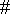
\includegraphics{hash-symbol}\kern-0.1em}
  \newcommand{\smallshp}{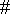
\includegraphics[scale=0.8]{hash-symbol}\kern-0.1em}
  \newcommand{\sharpsymbol}{\#}
  \newcommand{\shs}{\shp s}
  \newcommand{\shvs}{\shp vs}
  \newcommand{\smallshs}{\smallshp s}
  \newcommand{\sharpup}{\texttt{\sharpsymbol up}}
  \newcommand{\sharpdown}{\texttt{\sharpsymbol down}}
  % Sec 3.1 Truth
  \newcommand{\KPred}{\mathit{\shp Pred}}

  % Sec 3.2 Strings
  \newcommand{\KChar}{\texttt{\sharpsymbol Char}}
  \newcommand{\KCharList}{\texttt{\sharpsymbol CharList}}
  \newcommand{\KString}{\texttt{\sharpsymbol String}}
  \newcommand{\Kepsilon}{\texttt{\sharpsymbol epsilon}}
  \newcommand{\KconsKString}{\texttt{\sharpsymbol consKString}}

  %% We shouldn't need the follows.
  \newcommand{\Kconcat}{\texttt{\sharpsymbol concat}}

  \newcommand{\Kconstructor}{\texttt{\sharpsymbol constructor}}
  \newcommand{\KconstructorP}[1]{\parametric{\Kconstructor}{#1}}
  \newcommand{\Kinjective}{\texttt{\sharpsymbol injective}}
  \newcommand{\KinjectiveP}[1]{\parametric{\Kinjective}{#1}}

  \newcommand{\KprovableP}[1]{\parametric{\Kdeduce}{#1}}

  % Sec 3.3 Sorts and Symbols
  \newcommand{\KSort}{\texttt{\sharpsymbol Sort}}
  \newcommand{\Ksort}{\texttt{\sharpsymbol sort}}
  \newcommand{\KSymbol}{\texttt{\sharpsymbol Symbol}}
  \newcommand{\Ksymbol}{\texttt{\sharpsymbol symbol}}
  \newcommand{\KSymbolceil}{\texttt{\sharpsymbol `ceil}}
  \newcommand{\KgetArgumentSorts}{\texttt{\sharpsymbol getArgumentSorts}}
  \newcommand{\KgetReturnSort}{\texttt{\sharpsymbol getReturnSort}}

  % Sec 3.4 Finite Lists
  \newcommand{\ttX}{\texttt{X}}
  \newcommand{\ttChar}{\texttt{Char}}
  \newcommand{\ttSort}{\texttt{Sort}}
  \newcommand{\ttSymbol}{\texttt{Symbol}}
  \newcommand{\ttVariable}{\texttt{Variable}}
  \newcommand{\ttPattern}{\texttt{Pattern}}
  \newcommand{\XList}{\texttt{\sharpsymbol XList}}
  \newcommand{\KnilXList}{\texttt{\sharpsymbol nilXList}}
  \newcommand{\KconsXList}{\texttt{\sharpsymbol consXList}}
  \newcommand{\KappendXList}{\texttt{\sharpsymbol appendXList}}
  \newcommand{\KinXList}{\texttt{\sharpsymbol inXList}}
  \newcommand{\KdeleteXList}{\texttt{\sharpsymbol deleteXList}}
  \newcommand{\KPatternList}{\texttt{\sharpsymbol PatternList}}
  \newcommand{\KnilKPatternList}{\texttt{\sharpsymbol nilPatternList}}
  \newcommand{\KconsKPatternList}{\texttt{\sharpsymbol consPatternList}}
  \newcommand{\KappendKPatternList}{\texttt{\sharpsymbol appendPatternList}}
  \newcommand{\KinKPatternList}{\texttt{\sharpsymbol inPatternList}}
  \newcommand{\KdeleteKPatternList}{\texttt{\sharpsymbol deletePatternList}}
  \newcommand{\KSortList}{\texttt{\sharpsymbol SortList}}
  \newcommand{\KnilKSortList}{\texttt{\sharpsymbol nilSortList}}
  \newcommand{\KconsKSortList}{\texttt{\sharpsymbol consSortList}}
  \newcommand{\KappendKSortList}{\texttt{\sharpsymbol appendSortList}}
  \newcommand{\KinKSortList}{\texttt{\sharpsymbol inSortList}}
  \newcommand{\KdeleteKSortList}{\texttt{\sharpsymbol deleteSortList}}
  \newcommand{\KnilKSymbolList}{\texttt{\sharpsymbol nilSymbolList}}
  \newcommand{\KconsKSymbolList}{\texttt{\sharpsymbol consSymbolList}}
  \newcommand{\KSymbolList}{\texttt{\sharpsymbol SymbolList}}
  \newcommand{\KappendKSymbolList}{\texttt{\sharpsymbol appendSymbolList}}
  \newcommand{\KinKSymbolList}{\texttt{\sharpsymbol inSymbolList}}
  \newcommand{\KdeleteKSymbolList}{\texttt{\sharpsymbol deleteSymbolList}}
  \newcommand{\KnilKCharList}{\texttt{\sharpsymbol nilCharList}}
  \newcommand{\KconsKCharList}{\texttt{\sharpsymbol consCharList}}
  \newcommand{\KVariableList}{\texttt{\sharpsymbol VariableList}\xspace}
  \newcommand{\KnilKVariableList}{\texttt{\sharpsymbol nilVariableList}}
  \newcommand{\KconsKVariableList}{\texttt{\sharpsymbol consVariableList}}
  \newcommand{\KinKVariableList}{\texttt{\sharpsymbol inVariableList}}
  \newcommand{\KappendKVariableList}{\texttt{\sharpsymbol appendVariableList}}
  \newcommand{\KdeleteKVariableList}{\texttt{\sharpsymbol deleteVariableList}}
  \newcommand{\KappendKCharList}{\texttt{\sharpsymbol appendKCharList}}
  \newcommand{\KVariable}{\texttt{\sharpsymbol Variable}}
  \newcommand{\KVariableAsKPattern}{\texttt{\sharpsymbol variableAsPattern}}
  \newcommand{\KvariablePattern}{\texttt{\sharpsymbol variablePattern}}
  \newcommand{\KPattern}{\texttt{\sharpsymbol Pattern}}
  \newcommand{\Kvariable}{\texttt{\sharpsymbol variable}}
  \newcommand{\Kand}{\texttt{\sharpsymbol  \slashsymbol and}}
  \newcommand{\Kor}{\texttt{\sharpsymbol \slashsymbol  or}}
  \newcommand{\Kimplies}{\texttt{\sharpsymbol  \slashsymbol implies}}
  \newcommand{\Kiff}{\texttt{\sharpsymbol  \slashsymbol iff}}
  \newcommand{\Knot}{\texttt{\sharpsymbol  \slashsymbol not}}
  \newcommand{\Kapplication}{\texttt{\sharpsymbol application}}
  \newcommand{\Kexists}{\texttt{\sharpsymbol \slashsymbol  exists}}
  \newcommand{\Kforall}{\texttt{\sharpsymbol \slashsymbol  forall}}
  \newcommand{\Kequals}{\texttt{\sharpsymbol \slashsymbol  equals}}
  \newcommand{\Kmembership}{\Kin}
  \newcommand{\Kin}{\texttt{\sharpsymbol \slashsymbol  in}}
  \newcommand{\Kcontains}{\texttt{\sharpsymbol  \slashsymbol contains}}
  \newcommand{\Ktop}{\texttt{\sharpsymbol \slashsymbol  top}}
  \newcommand{\Kbottom}{\texttt{\sharpsymbol \slashsymbol  bottom}}
  \newcommand{\Kfloor}{\texttt{\sharpsymbol \slashsymbol  floor}}
  \newcommand{\Kceil}{\texttt{\sharpsymbol \slashsymbol  ceil}}
  \newcommand{\Knext}{\texttt{\sharpsymbol \slashsymbol next}}
  \newcommand{\Krewrites}{\texttt{\sharpsymbol \slashsymbol rewrites}}

  \newcommand{\KVariableListAsKPatternList}
    {\texttt{\sharpsymbol variableListAsPatternList}\xspace}

  \newcommand{\Kdv}{\texttt{\sharpsymbol \slashsymbol dv}}

  \newcommand{\KgetFV}{\texttt{\sharpsymbol getFV}}
  \newcommand{\KgetFVFromPatterns}{\texttt{\sharpsymbol getFVFromPatterns}}
  \newcommand{\KoccursFree}{\texttt{\sharpsymbol occursFree}}
  \newcommand{\KfreshName}{\texttt{\sharpsymbol freshName}}
  \newcommand{\Kcons}{\texttt{\sharpsymbol cons}}
  \newcommand{\Knil}{\texttt{\sharpsymbol nil}}
  \newcommand{\KSymbolzero}{\texttt{\sharpsymbol Symbolzero}}
  \newcommand{\KSymbolcons}{\texttt{\sharpsymbol Symbolcons}}
  \newcommand{\KSymbolnil}{\texttt{\sharpsymbol Symbolnil}}

  \newcommand{\KSignature}{\texttt{\sharpsymbol Signature}}
  \newcommand{\Ksignature}{\texttt{\sharpsymbol signature}}
  \newcommand{\KgetSorts}{\texttt{\sharpsymbol getSorts}}
  \newcommand{\KgetSymbols}{\texttt{\sharpsymbol getSymbols}}
  \newcommand{\KsortDeclared}[1]{
   \parametric{\texttt{\sharpsymbol sortDeclared}}{#1}}
  \newcommand{\KsortsDeclared}[1]{
        \parametric{\texttt{\sharpsymbol sortsDeclared}}{#1}}
  \newcommand{\KsymbolDeclared}[1]{
   \parametric{\texttt{\sharpsymbol symbolDeclared}}{#1}}
  \newcommand{\KaxiomDeclared}{\texttt{\sharpsymbol axiomDeclared}}
  \newcommand{\Kderivable}{\Kdeduce}

  \newcommand{\Ksubsort}[1]{\parametric{\texttt{\sharpsymbol subsort}}{#1}}
  \newcommand{\Ksubsorts}[1]{\parametric{\texttt{\sharpsymbol subsorts}}{#1}}
  \newcommand{\KSortConnectedComponent}{\texttt{\sharpsymbol
  SortConnectedComponent}}
  \newcommand{\KsubsortOverloading}[1]{
   \parametric{\texttt{\sharpsymbol subsortOverloading}}{#1}}

  \newcommand{\KwellFormed}{\texttt{\sharpsymbol wellFormed}}
  \newcommand{\KwellFormedPatterns}{\texttt{\sharpsymbol wellFormedPatterns}}
  \newcommand{\KgetSort}{\texttt{\sharpsymbol getSort}}
  \newcommand{\KgetSortsFromPatterns}{\texttt{\sharpsymbol
  getSortsFromPatterns}}
  \newcommand{\KisSort}{\texttt{\sharpsymbol isSort}}
  \newcommand{\Ksubstitute}{\texttt{\sharpsymbol substitute}}
  \newcommand{\KsubstitutePatterns}{\texttt{\sharpsymbol substitutePatterns}}

  \newcommand{\KTheory}{\texttt{\sharpsymbol Theory}}
  \newcommand{\Ktheory}{\texttt{\sharpsymbol theory}}
  \newcommand{\KwellFormedTheory}{\texttt{\sharpsymbol wellFormedTheory}}

  \newcommand{\Kdeduce}{\textup{\texttt{\sharpsymbol provable}}}

  \newcommand{\Ksc}[1]{\parametric{\textup{\texttt{\sharpsymbol sc}}}{#1}}

  % The italic font of "ceil" used in math mode.
  \newcommand{\cl}{\mathit{ceil}}

  \newcommand{\doublecolon}{::}
  % Use quotation marks "..." in math mode.
  \newcommand{\quot}[1]{\mathrm{``#1"}}
  \newcommand{\quottt}[1]{\textrm{\lq\texttt{#1}\rq}}
  \newcommand{\qquottt}[1]{\textrm{``\texttt{#1}''}}

  \newcommand{\Pattern}{\textsc{Pattern}\xspace}
  \newcommand{\ra}{\rightarrow}
  \newcommand{\lra}{\leftrightarrow}
  \newcommand{\FV}{{\it FV}}

  \newcommand{\name}{\mathit{name}}
  \newcommand{\llist}{\mathit{list}}
  \newcommand{\smalltt}[1]{\texttt{\small #1} }
  \newcommand{\sort}{\smalltt{sort}}
  \newcommand{\symb}{\smalltt{symbol}}
  \newcommand{\axiom}{\smalltt{axiom}}

  \newcommand{\inj}[2]{\parametric{\mathit{inj}}{#1, #2}}
  \newcommand{\retract}[2]{\parametric{\mathit{retract}}{#1, #2}}
  \newcommand{\factorial}{\textit{factorial}}
  % User-defined sorts & symbols in the meta-theory
  \newcommand{\KqNat}{\texttt{\shp `Nat}{ }}
  \newcommand{\KqList}{\texttt{\shp `List}{ }}
  \newcommand{\Kqzero}{\texttt{\shp `zero}{ }}
  \newcommand{\Kqsucc}{\texttt{\shp `succ}{ }}
  \newcommand{\Kqplus}{\texttt{\shp `plus}{ }}
  \newcommand{\Kqnil}{\texttt{\shp `nil}{ }}
  \newcommand{\Kqcons}{\texttt{\shp `cons}{ }}
  \newcommand{\Kqappend}{\texttt{\shp `append}{ }}
  \newcommand{\KqK}{\texttt{\shp `K}{}}
  \newcommand{\Kqinj}{\texttt{\shp `inj}}

  % Define the slash symbol
  \newcommand{\slashsymbol}{\symbol{92}}
  % Define slashed ttfamily words
  \newcommand{\slsh}[1]{\texttt{\slashsymbol#1}}
  \newcommand{\sland}{\slsh{and}}
  \newcommand{\slor}{\slsh{or}}
  \newcommand{\slnot}{\slsh{not}}
  \newcommand{\slimplies}{\slsh{implies}}
  \newcommand{\sliff}{\slsh{iff}}
  \newcommand{\slequals}{\slsh{equals}}
  \newcommand{\slexists}{\slsh{exists}}
  \newcommand{\slforall}{\slsh{forall}}
  \newcommand{\sltop}{\slsh{top}}
  \newcommand{\slbottom}{\slsh{bottom}}
  \newcommand{\slceil}{\slsh{ceil}}
  \newcommand{\slfloor}{\slsh{floor}}
  \newcommand{\slin}{\slsh{in}}
  \newcommand{\slnext}{\slsh{next}}
  \newcommand{\slrewrites}{\slsh{rewrites}}

  \newcommand{\sldv}{\slsh{dv}}

  \newcommand{\itlogic}{\mathit{logic}}
  \newcommand{\itconnective}{\mathit{connective}}
  \newcommand{\itsort}{\mathit{sort}}
  \newcommand{\itsymbol}{\mathit{symbol}}
  \newcommand{\itdeclared}{\mathit{declared}}
  \newcommand{\itsortDeclared}{\mathit{sortDeclared}}
  \newcommand{\collapse}{\mathit{collapse}}

  \newcommand{\ttv}{\texttt{v}}
  \newcommand{\ttp}{\texttt{p}}
  \newcommand{\itvp}{\mathit{vp}}

  \newcommand{\att}{\mathit{att}}
  \newcommand{\verbose}{\mathit{verbose}}
  \newcommand{\var}{\mathit{var}}

  \newcommand{\rand}{\mathsf{rand}}



  % Define syntactic category <category>
  \newcommand{\syntacc}[1]{\text{$\langle$\textit{#1}$\rangle$}}

  % Title and authors
  \title{Introduction to Matching Logic}
  \author{Runtime Verification}

\begin{document}

\maketitle

\tableofcontents

\section{Introduction}
\label{sec:introduction}

\K is a best effort realization of matching logic~\cite{rosu-2017-lmcs}.
Matching logic allows us to mathematically define arbitrarily infinite
theories, which are not in general possible to describe finitely.
\K proposes a finitely describable subset of matching logic theories.
Since its inception in 2003 as a notation within
Maude~\cite{clavel-et-al99a} convenient for teaching programming
languages~\cite{rosu-2003-cs322}, until recently \K's semantics was explained
either by translation to rewriting logic \cite{meseguer-1992-tcs} or by
translation to some form of graph rewriting~\cite{serbanuta-rosu-2012-icgt}.
These translations not only added clutter and came at a loss of part of the
intended meaning of \K, but eventually turned out to be a serious limiting
factor in the types of theories and languages that could be defined.
Matching logic was specifically created and developed to serve as a
logical, semantic foundation for \K, after almost 15 years of experience
with using \K to define the formal semantics of real-life programming
languages, including
C~\cite{ellison-rosu-2012-popl,hathhorn-ellison-rosu-2015-pldi},
Java~\cite{bogdanas-rosu-2015-popl},
JavaScript~\cite{park-stefanescu-rosu-2015-pldi},
Python~\cite{guth-2013-thesis,pltredex-python},
PHP~\cite{k-php},
EVM~\cite{hiraidefining,hildenbrandt-saxena-zhu-rodrigues-daian-guth-rosu-2017-tr}.

Matching logic allows us to define \emph{theories} $(S,\Sigma,A)$ consisting
of potentially infinite sets of \emph{sorts} $S$, of \emph{symbols}
$\Sigma$ over sorts in $S$ (also called $S$-symbols), and of \emph{patterns}
$A$ built with symbols in $\Sigma$ (also called $\Sigma$-patterns),
respectively, and provides models that interpret the symbols
relationally, which in turn yield a \emph{semantic validity} relation
$(S,\Sigma,A)\models\varphi$ between theories $(S,\Sigma,A)$ and
$\Sigma$-patterns $\varphi$.
Matching logic also has a Hilbert-style complete proof system, which allows
us to derive new patterns $\varphi$ from given theories $(S,\Sigma,A)$,
written $(S,\Sigma,A)\vdash\varphi$.
When the sorts and signature are understood, we omit them; for example,
the completeness of matching logic then states that for any matching logic
theory $(S,\Sigma,A)$ and any $\Sigma$-pattern $\varphi$, we have
$A \models \varphi$ iff $A \vdash \varphi$.

...\improvement{Will add more here as we finalize the notation.
we need some convincing example.  Maybe parametric maps?}
...\improvement{Bring some motivational arguments here why this is
all important.  Why do we want to define the semantics of \K by going
to the meta-level.  Why people who just want to implement \K tools should
be interested in this document.}

\section{Matching Logic}
\label{sec:matching-logic}

\newcommand{\Var}{\textit{Var}}
\newcommand{\Name}{\textit{Name}}

In this section we first recall basic matching logic syntax and semantics
notions from~\cite{rosu-2017-lmcs} at a theoretical level.


\subsection{Syntax}
\label{sec:ML-syntax}
Assume a matching logic \emph{signature} $(S, \Sigma)$, where $S$ is the
set of its \emph{sorts} and $\Sigma$ is the set of its \emph{symbols}.
When $S$ is understood, we write just $\Sigma$ for a signature instead of
$(S,\Sigma)$.
Assume a set {\Name} of infinitely many \emph{variable names}.
We partition $\Sigma$ in sets $\Sigma_{s_1 \ldots s_n, s}$, where
$s_1,\ldots, s_n, s \in S$.
The formulae of matching logic are called \emph{patterns}, although we
may also call them \emph{formulae}.
The set $\Pattern_s$ of patterns of sort $s \in S$ is generated by the
following grammar:
\begin{align*}
\varphi_s \Coloneqq\  &x \cln s \quad \text{where $x \in \Name$ and $s \in S$}
& \textrm{// variable}
\\
\mid\  &\sigma(\varphi_{s_1},...,\varphi_{s_n}) \quad\
\text{where $\sigma \in \Sigma_{s_1 \ldots s_n, s}$ and
$\varphi_{s_1},...,\varphi_{s_n}$ of appropriate sorts}
& \textrm{// structure}
\\
\mid\  &\varphi_s \wedge_s \varphi_s
& \textrm{// intersection}
\\
\mid\  &\neg_s \,\varphi_s
& \textrm{// complement}
\\
\mid\  &\exists_s \,x \cln s' .\, \varphi_s \quad \text{where $x \in N$ and $s' \in S$}
& \textrm{// binder}
\end{align*}
\begingroup\vspace*{-\baselineskip}
\captionof{figure}{The grammar of matching logic patterns.
For each $s\in S$, $\varphi_s$ are \emph{patterns of sort $s$}.}
\label{ml-grammar}
\vspace*{\baselineskip}\endgroup

Instead of writing $x \cln s$, we write just $x$ for a variable when $s$ is
understood from the context or irrelevant.
Similarly, we omit the subscript $s$ of $\wedge_s$, $\neg_s$, and respectively
$\exists_s$ when understood from context or irrelevant.
Given a symbol $\sigma \in \Sigma_{s_1 \ldots s_n,s}$, $s_1 \ldots s_n$ are
called the \emph{argument sorts} of $\sigma$, $s$ is called the
\emph{return sort} of $\sigma$, and $n$ is called the \emph{arity} of
$\sigma$.
By abuse of language, we take the freedom to identify symbols
$\sigma\in\Sigma_{s_1 \ldots s_n,s}$ with corresponding patterns
$\sigma(x_1\cln s_1,...,x_n\cln s_n)$, where $x_1$, ..., $x_n$ are all
distinct names.
When $n = 0$, we call $\sigma$ a \emph{constant symbol} or simply a
\emph{constant}.
If $\sigma$ is a constant, we write the pattern just $\sigma$ instead of
$\sigma()$ for
simplicity.

Let \Pattern be the $S$-sorted set of patterns $\{\Pattern_s\}_{s\in S}$.
The grammar above can be infinite, i.e., can have infinitely many
non-terminals and productions, because $S$ and $\Sigma$ can be
infinite.
Also, as usual, it only defines the syntax of formulae and not
their semantics.
For example, patterns $x \wedge y$ and $y \wedge x$ are distinct elements in
the language of the grammar, in spite of them being semantically/provably
equal in matching logic, as seen shortly.
For notational convenience, we take the liberty to use mix-fix syntax for
operators in $\Sigma$ and parentheses for grouping.
Also, recall that we may omit the sort of a variable when understood.
For example, if $\Nat \in S$ and
$\_+\_, \_*\_ \in \Sigma_{\Nat \times \Nat, \Nat}$
then we may write ``$(x + y)*z$'' instead of
``$\_*\_(\_+\_(x\cln\Nat,y\cln\Nat),z\cln\Nat)$''.
More notational conventions will be introduced along the way
as we use them.
We adopt the following derived constructs (``syntactic sugar''): %\vspace*{-1ex}
$$\begin{array}{rcl@{\hspace*{10ex}}rcl}
\top_{\!\!s} & \equiv & \exists x\!:\!s \,.\, x &
\varphi_1 \ra \varphi_2 & \equiv & \neg\varphi_1 \vee \varphi_2 \\
\bot_{s} & \equiv & \neg \top_{\!\!s} &
\varphi_1 \lra \varphi_2 & \equiv & (\varphi_1 \ra \varphi_2) \wedge
 (\varphi_2 \ra \varphi_1) \\
\varphi_1 \vee \varphi_2 & \equiv & \neg(\neg\varphi_1\wedge\neg\varphi_2) &
\forall x . \varphi & \equiv & \neg(\exists x . \neg\varphi) \\
%\varphi_1 = \varphi_2 & \equiv & \varphi_1 \lra \varphi_2
\end{array}
%\vspace*{-1ex}
$$
We adapt from first-order logic the notions of \emph{free variable}
($\FV(\varphi)$ is the set of free variables of $\varphi$) and of
variable-capture-free \emph{substitution} ($\varphi[\varphi'/x]$ denotes
$\varphi$ whose free occurrences of $x$ are replaced with $\varphi'$, possibly
renaming bound variables in $\varphi$ to avoid capturing free variables of
$\varphi'$).

A matching logic \emph{theory} is a triple $(S, \Sigma, A)$ where
$(S,\Sigma)$ is a signature and $A$ is a set of patterns called \emph{axioms}.
When $S$ is understood or not important, we write $(\Sigma,A)$ instead of $(S,\Sigma,A)$.

\subsection{Semantics and Basic Properties}
\label{sec:semantics}

A \emph{matching logic $(S,\Sigma)$-model} $M$ consists of:
An $S$-sorted set $\{M_s\}_{s\in S}$, where each set $M_s$,
called the \emph{carrier of sort $s$ of $M$}, is assumed
non-empty; and a function
$\sigma_M:M_{s_1}\times\cdots\times M_{s_n} \rightarrow {\cal P}(M_s)$
for each symbol $\sigma\in\Sigma_{s_1\ldots s_n,s}$, called the
\emph{interpretation} of $\sigma$ in $M$.
It is important to note that in matching logic symbols are interpreted as
functions into power-set domains, that is, as \emph{relations}, and not as
usual functions like in FOL.
We tacitly use the same notation $\sigma_M$ for its extension
to argument sets,
${\cal P}(M_{s_1})\times\cdots\times {\cal P}(M_{s_n}) \rightarrow {\cal P}(M_s)$.
When $S$ is understood we may call $M$ a \emph{$\Sigma$-model}, and when
both $S$ and $\Sigma$ are understood we call it simply a \emph{model}.
We let $\Mod(S,\Sigma)$, or $\Mod(\Sigma)$ when $S$ is understood, denote
the (category of) models of a signature $(S,\Sigma)$.
%
Given a model $M$ and a map
$\rho:\Var\rightarrow M$, called an \emph{$M$-valuation}, let its extension
$\overline{\rho}:\Pattern\rightarrow{\cal P}(M)$
be inductively defined as follows:\vspace*{-2ex}
\begin{itemize}\itemsep-1ex
\item $\overline{\rho}(x) = \{\rho(x)\}$, for all $x\in\Var_s$
\item $\overline{\rho}(\sigma(\varphi_{1},\ldots,\varphi_{n}))=
\sigma_M(\overline{\rho}(\varphi_1),\ldots \overline{\rho}(\varphi_n))$ for all
$\sigma\in\Sigma_{s_1...s_n,s}$ and appropriate $\varphi_1,...,\varphi_n$
%\item $\overline(\rho)(\top_{\!\!s}) = M_s$
\item $\overline{\rho}(\neg\varphi) = M_s \ \backslash\ \overline{\rho}(\varphi)$ for all
$\varphi\in\Pattern_s$
\item $\overline{\rho}(\varphi_1 \wedge \varphi_2) =
\overline{\rho}(\varphi_1) \cap \overline{\rho}(\varphi_2)$
for all $\varphi_1, \varphi_2$ patterns of the same sort
\item $\overline{\rho}(\exists x . \varphi) =
\bigcup\{\overline{\rho'}(\varphi) \mid \rho':\Var\rightarrow M,\
\rho'\!\!\upharpoonright_{\Var\backslash\{x\}} =
\rho\!\!\upharpoonright_{\Var\backslash\{x\}}\}
= \bigcup_{a\in M} \overline{\rho[a/x]}(\varphi)
$
\end{itemize}\vspace*{-.5ex}
where `` $\backslash$'' is set difference,
``$\rho\!\!\upharpoonright_V$'' is
$\rho$ restricted to $V \subseteq \Var$,
and ``$\rho[a/x]$'' is map $\rho'$ with $\rho'(x)=a$ and $\rho'(y)=\rho(y)$ if
$y\neq x$.
If $a\in \overline{\rho}(\varphi)$ then we say $a$ \emph{matches}
$\varphi$ (with witness $\rho$).

Pattern $\varphi_s$ is an \emph{$M$-predicate}, or a
\emph{predicate in $M$}, iff for any $M$-valuation $\rho:\Var\rightarrow M$,
it is the case that $\overline{\rho}(\varphi_s)$ is either $M_s$ (it holds) or
$\emptyset$ (it does not hold).
Pattern $\varphi_s$ is a \emph{predicate} iff it is a predicate in all
models $M$.
For example, $\top_s$ and $\bot_s$ are predicates, and if $\varphi$,
$\varphi_1$ and $\varphi_2$ are predicates then so are $\neg\varphi$,
$\varphi_1 \wedge \varphi_2$, and $\exists x\,.\,\varphi$.
That is, the logical connectives of matching logic preserve the predicate
nature of patterns.
A symbol $\sigma\in\Sigma_{s_1 \ldots s_n,s}$ is called a \emph{predicate} if
its corresponding pattern $\sigma(x_1\cln s_1,...,x_n\cln s_n)$ is a
predicate.

Model $M$ \emph{satisfies} $\varphi_s$, written ${M}\models \varphi_s$, iff
$\overline{\rho}(\varphi_s) = M_s$ for all $\rho:\Var\rightarrow M$.
Pattern $\varphi$ is \emph{valid}, written $\models \varphi$,
iff ${M} \models \varphi$ for all ${M}$.
If $A\subseteq\Pattern$ then ${M} \models A$ iff
${M} \models \varphi$ for all $\varphi\in A$.
$A$ \emph{entails} $\varphi$, written $A \models \varphi$,
iff for each ${M}$, ${M} \models A$ implies ${M} \models \varphi$.
We may subscript $\models$ with the signature whenever we feel it
clarifies the presentation; that is, we may write $\models_{(S,\Sigma)}$ or
$\models_\Sigma$ instead of $\models$.
A \emph{(matching logic) specification}, or a \emph{(matching logic) theory},
is a triple $(S,\Sigma,A)$, or just $(\Sigma,A)$ when $S$ is understood,
with $A$ a set of $\Sigma$-patterns.
We let $T$ range over specification/theories;
$T = (S,\Sigma,A)$ is \emph{finite} whenever $S$, $\Sigma$ and $A$ are finite.
Given specification $T=(S,\Sigma,A)$ we let $\Mod(T)$, or
$\Mod(S,\Sigma,A)$ or $\Mod(\Sigma,A)$, also denoted by $\denote{T}$,
or $\denote{(S,\Sigma,A)}$ or $\denote{(\Sigma,A)}$, be its (category of)
models $\{M \ \mid \ M \in \Mod_{\Sigma},\ M \models_{\Sigma} A \}$.

A signature $(S',\Sigma')$ is called a \emph{subsignature} of $(S,\Sigma)$, written
$(S',\Sigma') \hookrightarrow(S,\Sigma)$, if and only if $S' \subseteq S$ and
$\Sigma' \subseteq \Sigma$.
If $M \in \Mod(\Sigma)$ then we let
$\reduct{M}{\Sigma'} \in \Mod(\Sigma')$ denote its
\emph{$\Sigma'$-reduct}, or simply its \emph{reduct} when
$\Sigma'$ is understood, defined as follows:
$(\reduct{M}{\Sigma'})_{s'} = M_{s'}$ for any $s'\in S'$ and
$\sigma'_{\reductscript{M}{\Sigma'}} = \sigma'_M$ for any $\sigma'\in\Sigma'$.
It may help to think of signatures as interfaces and of models as
\emph{implementations} of such interfaces.
Indeed, models provide concrete values for each sort, and concrete relations
for symbols.
Then the reduct $\reduct{M}{\Sigma'}$ can be regarded as a ``wrapper'' of
the implementation $M$ of $\Sigma$ turning it into an implementation of
$\Sigma'$, or a reuse of a richer implementation in a smaller context.

\subsection{Useful Symbols and Notations}
\label{sec:useful}

Matching logic is rather poor by default.
For example, it has no functions, no predicates, no equality, and although
symbols are interpreted as sets and variables are singletons, it has no
membership or inclusion.
All these operations are very useful, if not indispensable in practice.
Fortunately, they and many others can be defined axiomatically in matching
logic.
That is, whenever we need these in order to define (the semantics of other
symbols in) a matching logic specification $(\Sigma,A)$, we can add
corresponding symbols to $\Sigma$ and corresponding patterns to $A$ as axioms,
so that, in models, the desired symbols or patterns associated to the
desired operations get interpreted as expected.

For any sorts $s_1,s_2\in S$, assume the following \emph{definedness}
symbol and corresponding pattern:
$$
\begin{array}{l@{\hspace*{7ex}}l}
\lceil\_\rceil_{s_1}^{s_2} \ \ \in \Sigma_{s_1,s_2}
& \textrm{// Definedness symbol} \\
\lceil x\!:\! s_1 \rceil_{s_1}^{s_2} \ \ \in A &
\textrm{// Definedness pattern}
\end{array}
$$
Like in many logics, free variables are assumed universally quantified.
So the definedness pattern axiom above should be read as
``$\forall x\cln s_1\,.\,\lceil x \rceil_{s_1}^{s_2}$''.
If $S$ is infinite, then we have infinitely many definedness symbols and patterns
above.
It is easy to show that if $\varphi \in \Pattern_{s_1}$ then
$\lceil\varphi\rceil_{s_1}^{s_2}$ is a predicate which holds iff $\varphi$ is
defined:
if $\rho : \Var \ra M$ then
$\overline{\rho}(\lceil\varphi\rceil_{s_1}^{s_2})$ is either $\emptyset$
(i.e., $\overline{\rho}(\bot_{s_2})$)
when $\overline{\rho}(\varphi) = \emptyset$
(i.e., $\varphi$ undefined in $\rho$), or is $M_{s_2}$
(i.e., $\overline{\rho}(\top_{s_2})$)
when $\overline{\rho}(\varphi) \neq \emptyset$ (i.e., $\varphi$ defined).

We also define \emph{totality}, $\lfloor\_\rfloor_{s_1}^{s_2}$, as a derived
construct dual to definedness:
$$
\begin{array}{lcl}
\lfloor\varphi\rfloor_{s_1}^{s_2}
& \equiv &
\neg\lceil\neg\varphi\rceil_{s_1}^{s_2}
\end{array}
$$
Totality also behaves as a predicate.
It states that the enclosed pattern is matched by all values.
That is, if $\varphi \in \Pattern_{s_1}$ then $\lfloor\varphi\rfloor_{s_1}^{s_2}$
is a predicate where if $\rho : \Var \ra M$ is any valuation
then $\overline{\rho}(\lfloor\varphi\rfloor_{s_1}^{s_2})$ is either $\emptyset$
(i.e., $\overline{\rho}(\bot_{s_2})$)
when $\overline{\rho}(\varphi) \neq M_{s_1}$
(i.e., $\varphi$ is not total in $\rho$), or is $M_{s_2}$
(i.e., $\overline{\rho}(\top_{s_2})$)
when $\overline{\rho}(\varphi) = M_{s_1}$
(i.e., $\varphi$ is total).

\emph{Equality} can be defined quite compactly using pattern totality and
equivalence.
For each pair of sorts $s_1$ (for the compared patterns) and
$s_2$ (for the context in which the equality is used), we define
$\_=_{s_1}^{s_2}\_$ as the following derived construct:
$$
\begin{array}{@{}rcll}
\varphi =_{s_1}^{s_2} \varphi' & \ \ \ \ \ \equiv \ \ \ \ \ &
\lfloor\varphi \lra \varphi'\rfloor_{s_1}^{s_2}
& \ \ \ \ \ \mbox{where } \varphi,\varphi' \in \Pattern_{s_1}
\end{array}
$$
Equality is also a predicate.
if $\varphi,\varphi' \in \Pattern_{s_1}$ and $\rho : \Var \ra M$ then
$\overline{\rho}(\varphi =_{s_1}^{s_2} \varphi') = \emptyset$
iff $\overline{\rho}(\varphi) \neq \overline{\rho}(\varphi')$, and
$\overline{\rho}(\varphi =_{s_1}^{s_2} \varphi') = M_{s_2}$
iff $\overline{\rho}(\varphi) = \overline{\rho}(\varphi')$.

Similarly, we can define \emph{membership}:
if $x\in\Var_{s_1}$, $\varphi\in\Pattern_{s_1}$ and $s_1,s_2\in S$, then
let
$$
\begin{array}{@{}rcll}
x \in_{s_1}^{s_2} \varphi & \ \ \ \ \ \equiv \ \ \ \ \ &
\lceil x \wedge \varphi\rceil_{s_1}^{s_2}
& % \ \ \ \ \ \mbox{where } x \in \Var_{s_1},\varphi\in \Pattern_{s_1}\\
\end{array}
$$
Membership is also a predicate.
Specifically, for any $\rho:\Var\ra M$,
$\overline{\rho}(x \in_{s_1}^{s_2} \varphi) = \emptyset$
iff $\rho(x) \not\in \overline{\rho}(\varphi)$, and
$\overline{\rho}(x \in_{s_1}^{s_2} \varphi) = M_{s_2}$
iff $\rho(x) \in \overline{\rho}(\varphi)$.
It is convenient to extend the definition of membership to cases when the first
component is not a variable, but a pattern:
if $\psi, \varphi \in \Pattern_{s_1}$, and $s_1,s_2\in S$,
then let
$$
\begin{array}{@{}rcll}
\psi \in_{s_1}^{s_2} \varphi & \ \ \ \ \ \equiv \ \ \ \ \ &
\lceil \psi \wedge \varphi\rceil_{s_1}^{s_2}
& % \ \ \ \ \ \mbox{where } x \in \Var_{s_1},\varphi\in \Pattern_{s_1}\\
\end{array}
$$
This allows a uniform interface for pattern constructs, which yields neat
implementation of operations such as substitution.
As an example, consider $\varphi_1[\varphi_2 / x]$ where we
substitute $x$ for $\varphi_2$ in $\varphi_1$.
If the membership construct only accept variables as its first component, then
the substitution is only defined when $x$ does not occur free in the first
component of any membership construct in $\varphi_1$, and any implementation of
substitution will have to take that into account and perform an
``occurs check'' for $x$ in $\varphi_1$, and this could be expensive.

When writing patterns, the following precedence and associativity rules are
useful to reduce the
number of necessary parentheses.
\begin{center}
 \begin{tabular}{c|c|c}
  Connective      &     Precedence & Associativity \\\hline
  $\neg$          &     1          &  --           \\\hline
  $=$, $\in$      &     2          &  --           \\\hline
  $\wedge$        &     3          &  left         \\\hline
  $\vee$          &     4          &  left         \\\hline
  $\to$           &     5          &  right        \\\hline
  $\leftrightarrow$ &   6          &  --           \\\hline
  $\exists$,$\forall$ & 7          &  --           \\\hline
 \end{tabular}
\end{center}
As a convention, binders ($\forall$ and $\exists$) have a lower precedence than
other connectives.
This means that the scope of a binder extends as far to the right as possible.

Since $s_1$ and $s_2$ can usually be inferred from context,
we write $\lceil\_\rceil$ or $\lfloor\_\rfloor$ instead of
$\lceil\_\rceil_{s_1}^{s_2}$ or $\lfloor\_\rfloor_{s_1}^{s_2}$, respectively,
and similarly for the equality and membership.
Also, if the sort decorations cannot be inferred from context, then we assume
the stated property/axiom/rule holds for all such sorts.
\info{Refer to this later when we talk about parameters.}
%
For example, the generic pattern axiom ``$\lceil x \rceil$ where $x\in\Var$''
replaces all the axioms $\lceil x\!:\!s_1 \rceil_{s_1}^{s_2}$ above for all
the definedness symbols for all the sorts $s_1$ and $s_2$.

Note that, by default, symbols are interpreted as relations in matching logic.
It is often the case, though, that we want symbols to be interpreted as
(partial or total) \emph{functions}.
This can be easily done by axiomatically constraining those symbols to evaluate to
singletons.
For example, if $f$ is a unary symbol, then the pattern equation
``$\forall x\,.\,\exists y\,.\,f(x) = y$'' (the convention for free variables
allows us to drop the universal quantifier) states that in any model
$M$, the set $f_M(a)$ contains precisely one element for any $a\in M$;
i.e. $f$ is a total function.
Likewise, ``$\forall x\,.\,\exists y\,.\,\lceil f(x) \rceil \rightarrow f(x) = y$''
states that $f_M(a)$ contains at most one element ($f$ is a partial function).
%
Inspired from similar notations in other logics,
we adopt the familiar notation
``$\sigma : s_1 \times \cdots \times s_n \ra s$''
to indicate that $\sigma$ is a symbol in $\Sigma_{s_1\ldots s_n,s}$ and that
the pattern
$
\exists y\,.\,\sigma(x_1,\ldots,x_n) = y
$ is in $A$.
In this case, we call $\sigma$ a \emph{function symbol} or even just a
\emph{function}.
Patterns built with only function symbols are called
\emph{term patterns}, or simply just \emph{terms}.
The functionality property can be extended from a symbol to
a pattern: equation ``$\exists y\,.\,\varphi = y$'' states that pattern
$\varphi$ is \emph{functional}; it is easy to see that terms are
functional patterns.
Partial functions and total relations can also be axiomatized;
we refer the interested reader to \cite{rosu-2017-lmcs}.

\emph{Constructors} can also be axiomatized in matching logic.
Constructors play a critical role in programming language semantics,
because they can be used to build programs, data, as well as semantic
structures to define and reason about languages and programs.
The main characterizing properties of constructors are ``no junk''
(i.e., all elements are built with constructors) and ``no confusion''
(i.e., all elements are built in a unique way using constructors),
which can both be defined axiomatically in matching logic.
Specifically, let us fix a sort $s$ and suppose that we want to state
that the finite set of symbols
$\{c_i \in \Sigma_{s_i^1...s_i^{m_i},s} \ \mid \ 1 \leq i \leq n\}$
are constructors for $s$.
Then

\begin{description}
\item[No junk:]
We require that $A$ contain, or entail, the following pattern
$$
\bigvee_{i=1}^n \exists x_i^1:s_i^1\dots\exists x_i^{m_i}:s_i^{m_i}\ .\
c_i(x_i^1,\dots,x_i^{m_i})
$$
This states that any element of sort $s$ is in the image of at least one of
the constructors.

\item[No confusion, different constructors:]
For any $1 \leq i \neq j \leq n$, $A$ contains or entails
$$
\neg(c_i(x_i^1,\dots,x_i^{m_i}) \wedge c_j(x_j^1,\dots,x_j^{m_j}))
$$
This states that no element is in the image of two different constructors.
\item[No confusion, same constructor:] For any $1\leq i\leq n$, $A$ contains
or entails
$$
c_i(x_i^1,\dots,x_i^{m_i}) \wedge
c_i(y_i^1,\dots,y_i^{m_i}) \ra
c_i(x_i^1 \wedge y_i^1,\dots,x_i^{m_i}\wedge y_i^{m_i})
$$
This states that each element is constructed in a unique way.
That follows because for any two variables $x$ and $y$ of same sort,
$x \wedge y$ is interpreted as either a singleton set when $x$ and $y$
are interpreted as the same element, or as the empty set otherwise.
\end{description}
Additionally, if each $c_i$ is functional, then we call them
\textbf{functional constructors}.
The usual way to define a set of constructors is to have $A$
include all the patterns above.

An interesting observation is that \emph{unification} and, respectively,
\emph{anti-unification} (or \emph{generalization},
can be regarded as conjunction and, respectively, as disjunction of
patterns~\cite{rosu-2017-lmcs}.

\subsection{Sound and Complete Deduction}
\label{sec:deduction}

\newcommand{\sequent}[2]{{#1}\vdash{#2}}

Our proof system is a Hilbert-style proof system (not to be confused with a
Gentzen-style proof system).
To avoid any confusion about our notation and to remind the reader the
basics of axiom and proof rule \emph{schemas}, we start by briefly recalling
what a Hilbert-style proof system is, but for specificity we do it in the
context of matching logic.
A \emph{proof rule} is a pair $(\{\varphi_1,...,\varphi_n\},\varphi)$,
written
$$
\frac{
\varphi_1 \ \ ... \ \ \varphi_n
}{\varphi}
$$
The formulae $\varphi_1$, ..., $\varphi_n$ are called the \emph{hypotheses}
and $\varphi$ is called the \emph{conclusion} of the rule.
The order in which the hypotheses occur in a proof rule is irrelevant.
When $n = 0$ we call the proof rule an \emph{axiom} and take the freedom to
drop the empty hypotheses and the separating line, writing it simply as
``$\varphi$''.
A proof system allows us to \emph{formally prove} or \emph{derive} formulae.
Specifically, for any given finite or infinite specification $(\Sigma,A)$,
a proof system yields a \emph{provability relation},
written $\sequent{A}{\varphi}$, defined inductively as follows:

$\sequent{A}{\varphi}$ if $\varphi \in A$; and

$\sequent{A}{\varphi}$ if there is a proof rule like above such that
$\sequent{A}{\varphi_1}$, ..., $\sequent{A}{\varphi_n}$.

\noindent
Formulae in $A$ can therefore be regarded as axioms, and we even take the
freedom to call them axioms when there is no misunderstanding.
However, note that a proof system is fixed for the target logic, including
all its axioms (i.e., proof rules with no hypotheses).
We use the notation $T \vdashfin \varphi$ or $A \vdashfin \varphi$ to
emphasize the fact that the theory $T$ or the set of axioms $A$ is finite.

Proof systems can be and typically are infinite, that is, contain infinitely
many proof rules.
To write them using finite resources (space, time), we make use of \emph{proof schemas}
and \emph{meta-variables}.
As an example, let us recall the usual proof system of propositional logic,
which is also included in the proof system we propose here for matching logic:

\vspace*{2ex}

\noindent
\underline{Propositional calculus proof rules:}

\begin{quote}
1. $\varphi_1 \ra (\varphi_2 \ra \varphi_1)$
\hfill \textsc{(Propositional$_1$)}
\end{quote}

\begin{quote}
2. $(\varphi_1 \ra (\varphi_2 \ra \varphi_3)) \ra ((\varphi_1 \ra \varphi_2) \ra (\varphi_1 \ra \varphi_3))$
\hfill \textsc{(Propositional$_2$)}
\end{quote}

\begin{quote}
3. $(\neg \varphi_1 \ra \neg\varphi_2) \ra (\varphi_2 \ra \varphi_1)$
\hfill \textsc{(Propositional$_3$)}
\end{quote}

\begin{quote}
4. $\displaystyle\frac{\varphi_1 \ \ \ \ \varphi_1 \ra \varphi_2}{\varphi_2}$
\hfill \textsc{(Modus Ponens)}
\end{quote}

In propositional logic, $\varphi_1$, $\varphi_2$ and $\varphi_3$ above are
meta-variables ranging over propositions.
The first three are \emph{axiom schemas} while the fourth is a proper
\emph{rule schema}.
Schemas can be regarded as templates, which specify infinitely many instances,
one for each instance of the meta-variables.
We take the four proof rule schemas of propositional logic unchanged and
regard them as proof rule schemas for matching logic.
Note, however, that the \emph{meta-variables now range over patterns} of
the same sort, and thus there is a schema for each sort.

Matching logic also includes some of the proof rules
that deal with quantifiers from first order logic.
Notice that as explained in \cite{rosu-2017-lmcs},
the FOL substitution proof rule
does not hold in its general form in matching logic.
Instead, we only have
\emph{variable substitution} in matching logic.

\vspace*{2ex}

\noindent
\underline{First-order logic proof rules:}

\begin{quote}
5. $\vdash (\forall x\,.\,\varphi_1\ra\varphi_2) \ra (\varphi_1 \ra \forall x\,.\,\varphi_2)$
when $x\not\in\FV(\varphi_1)$
\hfill \textsc{($\forall$)}
\end{quote}

\begin{quote}
6. $\displaystyle\frac{\varphi}{\forall x\,.\,\varphi}$
\hfill \textsc{(Universal Generalization)}
\end{quote}

\begin{quote}
7. $\vdash (\forall x\,.\,\varphi) \ra \varphi[y/x]$
\hfill \textsc{(Variable Substitution)}
\end{quote}

In addition to the above rules borrowed from FOL, matching
logic also introduces the following rules for (reasoning about) structures.

\vspace*{2ex}

\noindent
\underline{Propagation rules:}

\begin{quote}
8. $\vdash \sigma(\varphi_1 \ddd \varphi_{i-1}, \bot,
                  \varphi_{i+1} \ddd \varphi_n)
           \imp \bot$
\hfill \textsc{(Propagation$_\bot$)}
\end{quote}

\begin{quote}
9.
$
\begin{array}{l}
\sigma(
\varphi_1 \ddd \varphi_{i-1},
\varphi_i \vee \varphi'_i,
\varphi_{i+1} \ddd \varphi_n) \imp
\\
\sigma(\varphi_1 \ddd \varphi_{i-1}, \varphi_i,
\varphi_{i+1} \ddd \varphi_n)
\\
\vee
\sigma(\varphi_1 \ddd \varphi_{i-1}, \varphi'_i,
\varphi_{i+1} \ddd \varphi_n)
\end{array}
$
\hfill \textsc{(Propagation$_\vee$)}
\end{quote}

\begin{quote}
10.
$
\begin{array}{l}
\sigma(
\varphi_1 \ddd \varphi_{i-1},
\exists x . \varphi_i,
\varphi_{i+1} \ddd \varphi_n) \imp
\\
\exists x .
\sigma(\varphi_1 \ddd \varphi_{i-1}, \varphi_i,
\varphi_{i+1} \ddd \varphi_n)
\end{array}
$
when $x \not\in \bigcup_{j \neq i} \FV(\varphi_j)$
\hfill \textsc{(Propagation$_\exists$)}
\end{quote}

\vspace*{2ex}

\noindent
\underline{Frame rule:}

\begin{quote}
 11.
 $\displaystyle\frac{\varphi_i \imp \varphi'_i}
 {\sigma(\varphi_1 \ddd \varphi_{i-1} ,
  \varphi_i,
  \varphi_{i+1} \ddd \varphi_n)
  \imp
  \sigma(\varphi_1 \ddd \varphi_{i-1} ,
  \varphi'_i,
  \varphi_{i+1} \ddd \varphi_n)
 }$
 \hfill \textsc{(Framing)}
\end{quote}

Besides the above rules, we need two more proof rules
to make the proof system a complete one.
These two rules are

\vspace*{2ex}

\noindent
\underline{More rules:}

\begin{quote}
 12.
 $\vdash \exists x . x$
 \hfill \textsc{(Existence)}
\end{quote}

To ease our notation in writing the next proof rule,
let us introduce \emph{symbol context}.
We abbreviate
$\sigma(\varphi_1 \ddd \varphi_{i-1}, \varphi_i,
        \varphi_{i+1} \ddd \varphi_n)$
as $\Csigmaiapp{\varphi_i}$.
When the position $i$ is not important,
we omit it and write $\Csigmaapp{\varphi_i}$.
We inductively define what a \emph{symbol context} is.
A symbol context $C$ is either the identity context, i.e.,
$C[\varphi] = \varphi$,
or $C[\varphi] = \Csigmaapp{C'[\varphi]}$
where $C'$ is a symbol context.
In other words, $C[\varphi]$ is a symbol context if
the path of the occurrence of $\varphi$ in $C[\varphi]$
contains only symbols and no logic connectives.

Using our notation of symbol contexts, we present the last proof rule
which captures the fact that variables are singletons:

\begin{quote}
 13.
 $\vdash \neg ( C_1[x \wedge \varphi]
  \wedge C_2[ x \wedge \neg \varphi ] )$
 where $C_1, C_2$ are symbol contexts
 \hfill \textsc{(Singleton Variables)}
\end{quote}

The following result establishes the soundness and completeness
of the proof system above:

\begin{theorem}\cite{rosu-2017-lmcs}
\label{thm:completeness}
For any matching logic specification $(\Sigma,A)$ and $\Sigma$-pattern
$\varphi$, $A \models \varphi$ iff $\sequent{A}{\varphi}$.
\end{theorem}

Note that Theorem~\ref{thm:completeness} also holds when the matching logic
specification is infinite, that is, when it has infinitely many sorts and
symbols in $\Sigma$ and infinitely many axioms in $A$.


\section{Important Case Studies}
\label{sec:case-studies}

In this section we illustrate the power of matching logic by showing how it can
handle binders, fixed-points, contexts, and rewriting and reachability.
These important notions or concepts can be defined as syntactic sugar or as
particular theories in matching logic, so that the uniform matching logic proof
system in Section~\ref{sec:deduction} can be used to reason about all of these.
In particular, \K can now be given semantics fully in matching logic.
That is, a \K language definition becomes a matching logic theory, and the
various tools that are part of the \K framework become best-effort
implementations of targeted proof search using the deduction system in
Section~\ref{sec:deduction}.

\subsection{Binders}
\label{sec:binders}

\info[inline]{More recent research shows that binders can be defined as
functional symbols. Change section 4.1--4.3 to reflect that.}

The \K framework allows to define binders, such as the $\lambda$ binder in
$\lambda$-calculus, using the attribute \texttt{binder}.
But what does that really mean?
Matching logic appears to provide no support for binders, except for having
its own binder, the existential quantifier $\exists$.
Here we only discuss untyped $\lambda$-calculus, but the same ideas apply to
any calculus with binders.

Suppose that $S$ consists of only one sort, $\Exp$, for $\lambda$-expressions.
Although matching logic provides an infinite set of variables $\Var_\Exp$ of
sort $\Exp$, we cannot simply define $\lambda\_.\_$ as a symbol in
$\Sigma_{\Var_\Exp \times \Exp, \Exp}$, for at least two reasons:
first, $\Var_\Exp$ is \emph{not} an actual sort at the core level
(as seen in Section~\ref{sec:meta-theory}, it is a sort at the meta-level);
second, we want the first argument of $\lambda\_.\_$ to bind its occurrences
in the second argument, and symbols do not do that.
To ease notation, from here on in this section assume that all variables
are in $\Var_\Exp$ and all patterns have sort $\Exp$.

The key observation here is that the $\lambda\_.\_$ construct in
$\lambda$-calculus \emph{performs two important operations}: on the one hand
it builds a binding of its first argument into its second, and on the other
hand it builds a term.
Fortunately, matching logic allows us to separate these two operations, and
use the builtin existential quantifier for binding.
Specifically, we define a symbol $\lambda^0$ and regard $\lambda$ as syntactic
sugar for the pattern that existentially binds its first argument into $\lambda^0$:
$$
\begin{array}{l}
\lambda^0 \in \Sigma_{\Exp\times\Exp,\Exp} \\
\lambda x . e \equiv \exists x . \lambda^0(x,e)
\end{array}
$$
Therefore, $\lambda^0(x,e)$ builds a term (actually a pattern) with no binding
relationship between the its first argument $x$ and other occurrences of $x$ in
term/pattern $e$, and then the existential quantifier $\exists x$ adds the binding
relationship.\improvement{Explain why $\lambda$ is not a symbol, but an alias}
Mathematically, we can regard $\lambda^0$ as constructing points (input, output)
on the graph of the function, and then the existential quantifier gives us their
union as stated by its matching logic semantics, that is, the actual function.
Note that this same construction does not work in FOL, because there quantifiers
apply to predicates and not to terms/patters.
It is the very nature of matching logic to not distinguish between function
and predicate symbols that makes the above work.
The application can be defined as an ordinary symbol:
$$
\_\,\_ \in \Sigma_{\Exp \times \Exp,\Exp}
$$

Let us now discuss the axiom patterns.
First, note that we get the $\alpha$-equality property,
$$
\lambda x . e = \lambda y . e[y/x]
$$
essentially for free, because matching logic's builtin existential quantifier
and substitution already enjoy the $\alpha$-equivalence
property~\cite{rosu-2017-lmcs}.
The $\beta$-equality, on the other hand, requires an important side condition.
To start the discussion, let us suppose that we naively define it as follows:
$$
\begin{array}{r@{\hspace*{4ex}}l}
(\lambda x . e)e' = e[e'/x]
&
\textrm{for any \emph{pattern} $e$ \ \ \ \ \doubleslash this is actually wrong!}
\end{array}
$$
The problem is that $e$ and $e'$ cannot be just any arbitrary patterns.
For example, if we pick $e$ to be $\top$ and $e'$ to be $\bot$, then
we can show that $(\lambda x . \top)\bot = \bot$
(see Section~\ref{sec:semantics}: the interpretation of $\_\,\_$ is empty
when any of its arguments is empty), and since $\top[\bot/x] = \top$ we
get $\top = \bot$, that is, inconsistency.
Matching logic, therefore, provides patterns that were not intended for
$\lambda$-calculus.
The solution is to restrict, with side conditions, the application of
$\beta$-equality to only patterns that correspond to $\lambda$-terms
in the original calculus:
$$
\begin{array}{r@{\hspace*{4ex}}l}
(\lambda x . e)e' = e[e'/x]
& \textrm{where $e$, $e'$ are patterns constructed only with variables}
\\
& \textrm{$\lambda$ binders (via desugaring) and application symbols}
\end{array}
$$
That is, we first identify a syntactic fragment of the universe of
patterns which is in a bijective correspondence with the original
syntactic terms of $\lambda$-calculus, and then restrict the
application of the $\beta$-equality rule to only patterns in that
fragment.

The above gives us an embedding of $\lambda$-calculus as a theory
in matching logic.
We conjecture that this embedding is a \emph{conservative extension},
that is, if $e$ and $e'$ are two $\lambda$-terms, then $e=e'$ holds
in the original $\lambda$-calculus if and only if the corresponding
equality between patterns holds in the matching logic theory.
The ``only if'' part is easy, because equational reasoning is sound
for matching logic~\cite{rosu-2017-lmcs}, but the ``if'' part appears
to be non-trivial.


\subsection{Fixed Points}
\label{sec:fixed-points}

Similarly to the $\lambda$-binder in Section~\ref{sec:binders}, we can
add a fixed-point $\mu$-binder as follows:
$$
\begin{array}{r@{\hspace*{4ex}}l}
\mu^0 \in \Sigma_{\Exp\times\Exp,\Exp}
\\
\mu x . e \equiv \exists x . \mu^0(x,e)
\\
\mu x . e = e[\mu x.e/x]
& \textrm{where $e$ is a pattern corresponding to a term}
\\
& \textrm{in the original calculus (i.e., constructed with variables,}
\\
& \textrm{$\lambda$ and $\mu$ binders (via desugaring), and application
symbols)}
\end{array}
$$
Given any model $M$ and interpretation $\rho : \Var \ra M$, pattern $e$
yields a function $e_M : M \rightarrow {\cal P}(M)$ where
$e_M(a) = \overline{\rho[a/x]}(e)$.
It is easy to see that its point-wise extension
$e_M : {\cal P}(M) \rightarrow {\cal P}(M)$ is monotone w.r.t. $\subseteq$,
so by the Knaster-Tarski theorem it has a fixed point\footnote{
Moreover, the set of fixed-points of
$e_M : {\cal P}(M) \rightarrow {\cal P}(M)$ forms a complete lattice.}.
In fact, if we let $X$ be the set $\overline{\rho}(\mu x . e)$, then
the equation of $\mu$ above yields $X = e_M(X)$, that is, $X$ is a fixed point
of $e_M : {\cal P}(M) \rightarrow {\cal P}(M)$.
%
We want, however, $X$ to be the \emph{least} fixed-point of $e_M$.
This is not possible in general, because $M$ and $\rho$ are arbitrary
and many of the fixed-points of $e_M$, including the least fixed-point,
may very well be unreachable with patterns.
However, from a practical perspective, the importance of those syntactically
unreachable fixed-points is questionable.
Considering that when we do proofs we can only derive patterns, it makes
sense to limit ourselves to only fixed points that can be expressed
syntactically.
Within this limited universe, we can axiomatize the syntactic
\emph{least fixed-point} nature of $\mu x . e$ with the following
pattern schema, which we call ``Knaster-Tarski'':\info{Explain why only
implication suffices in the LHS.}
$$
\begin{array}{r@{\hspace*{4ex}}l}
\floor{e[e'/x] \rightarrow e'} \rightarrow \floor{\mu x . e \rightarrow e'}
& \textrm{where $e$ and $e'$ are patterns corresponding to terms}
\\
& \textrm{in the original calculus}
\end{array}
$$

It is now a simple exercise to add a dual, greatest fixed-point construct:
$$
\begin{array}{r@{\hspace*{4ex}}l}
\nu^0 \in \Sigma_{\Exp\times\Exp,\Exp}
\\
\nu x . e \equiv \exists x . \nu^0(x,e)
\\
\nu x . e = e[\nu x.e/x]
& \textrm{where $e$ is a pattern corresponding to a term}
\\
& \textrm{in the original calculus} \\
\floor{e' \rightarrow e[e'/x]} \rightarrow \floor{e' \rightarrow \nu x . e}
& \textrm{where $e$ and $e'$ are patterns corresponding to terms}
\\
& \textrm{in the original calculus}
\end{array}
$$

\info{An alternative is to define $\nu x . e$ directly as the dual of
$\mu x . e$, that is, $\nu x . e \equiv \neg \mu x . \neg e$.
Can we prove the pattern above then?}

We extend our conjecture in Section~\ref{sec:binders} and conjecture
that the embedding above, in spite of not necessarily yielding the
expected absolute least fixed-points in all models (but least only
relatively to patterns that can be constructed with the original
syntax), remains a conservative extension: if $e$ and $e'$ are two
terms built with the syntax of the original calculus, then $e=e'$
holds in the original calculus if and only if the corresponding equality holds
in the corresponding matching logic theory.
Like before, the ``only if'' part is easy.

An alternative way to define greatest fixed-point is using the least fixed-point construct:
\begin{align*}
\nu x . e \equiv \neg \mu x . (\neg e[\neg x / x])
\end{align*}
where the pattern $\neg e[\neg x / x]$ is called the \emph{dual of pattern $e$ w.r.t. the variable $x$}.
This definition is justified by the following theorem which establishes the duality between least and greatest fixed-points.
\begin{theorem}[Duality of Fixed-Points]
 Let $F \colon 2^M \to 2^M$ be a monotone function. By Knaster-Tarski theorem,
 it has a unique least fixed-point $\mu x . F \subseteq M$ and a unique
 greatest fixed-point $\nu x . F \subseteq M$, which satisfy the following
 duality equations:
 \begin{align*}
 & \nu x . F = M \setminus \left( \mu x . \bar{F} \right) \\
 & \mu x . F = M \setminus \left( \nu x . \bar{F} \right) \\
 \end{align*}
 where $\bar{F} \colon 2^M \to 2^M$ is also a monotone function defined as
 $\bar{F}(A) = M \setminus ( F(M \setminus A))$.
\end{theorem}

\subsection{Contexts}

Matching logic allows us to define a very general notion of context.
Our contexts can be used not only to define evaluation strategies of
various language constructs, like how evaluation contexts are
traditionally used~\cite{felleisen-hieb-92}, but also for configuration
abstraction to enhance modularity and reuse, and for matching multiple
sub-patterns of interest at the same time.
\unsure{Brandon: how about the locality principle?}

Like $\lambda$ in Section~\ref{sec:binders}, contexts are also defined
as binders.
However, they are defined as schemas parametric in the sorts of their
hole and result, respectively, and their application is controlled by
their structure and surroundings.
We first define the generic infrastructure for contexts:
$$
\begin{array}{r@{\hspace*{5ex}}l}
\parametric{\Context}{s,s'} &
\textrm{sort schema, where $s$ (hole sort) and}
\\ &\textrm{$s'$ (result sort) range over any sorts}
\\ \parametric{\gamma^0}{s,s'} \in \Sigma_{s \times s',
\parametricscript{\Context}{s,s'}}
& \textrm{symbol schema, for all sorts $s, s'$}
\\ \parametric{\gamma\_.\_}{s,s'}(\hole\cln s,T\cln s') \equiv \exists \hole .
\parametric{\gamma^0}{s,s'}(\hole,T)
& \textrm{here, $\hole$ is an ordinary variable}
\\
\parametric{\_[\_]}{s,s'} \in \Sigma_{\parametricscript{\Context}{s,s'} \times s, s'}
& \textrm{symbol schema, for all sorts $s, s'$}
\\
\parametric{\_[\_]}{s,s}(\parametric{\gamma\_.\_}{s,s}(\hole\cln s, \hole),T\cln s) = T
& \textrm{axiom schema for identity contexts, for all sorts $s$}
\end{array}
$$
And the following axiom schema for composing nested contexts:
\begin{align*}
&\parametric{\_[\_]}{s',s''}(C_1 \cln \parametric{\Context}{s',s''},
\parametric{\_[\_]}{s,s'}(C_2 \cln \parametric{\Context}{s,s'},
T\cln s))
\\
= &
\parametric{\_[\_]}{s,s''}(
\parametric{\gamma\_.\_}{s,s''}(\hole\cln s,
\parametric{\_[\_]}{s',s''}(
C_1 \cln \parametric{\Context}{s',s''},
\parametric{\_[\_]}{s,s'}(C_2 \cln \parametric{\Context}{s,s'},
\hole\cln s))
), T\cln s)
\end{align*}
The sort parameters of axiom schemas can usually be inferred from the context.
To ease notation, from here on we assume they can be inferred and apply the
mixfix notation for symbols containing ``$\_$'' in their names.
With these, the last two axiom schemas above become:
\begin{align*}
& (\gamma \hole .\; \hole)[T] = T \\
& C_1[C_2[T]] = (\gamma \hole . C_1[C_2[\hole]])[T]
\end{align*}
We write
$C_1 \compose C_2 \equiv \gamma \hole . C_1[C_2[\hole]]$
for nested context.
Using this notation, the last axiom becomes
$$
C_1[C_2[T]] = (C_1 \compose C_2) [T]
$$

The above sort, symbol and axiom schemas are generic and tacitly assumed in
all definitions that make use of contexts.
Let us now illustrate specific uses of contexts.

\subsubsection{Evaluation Strategies of Language Constructs}
\label{sec:evaluationstrategies}
Suppose that a programming language has an if-then-else statement,
say $\ite\in\Sigma_{\BExp\times\Stmt\times\Stmt,\Stmt}$,
whose evaluation strategy is to first evaluate its first argument and then, depending
on whether it evaluates to $\ttrue$ or $\ffalse$, to rewrite to either
its second argument or its third argument.
We here only focus on its evaluation strategy and not its reduction rules;
the latter will be discussed in Section~\ref{sec:rewriting}.
Assuming that all reductions/rewrites apply in context, as discussed in
Section~\ref{sec:rewriting}, we can state that $\ite$ is given permission to
apply reductions within its first argument with the following axiom:
$$
\ite(T,S_1,S_2) = (\gamma\hole.\;\ite(\hole,S_1,S_2))[T]
$$
In practice, the above equation is often oriented as two rewrite rules.
The rewrite rule from left to right is called \emph{heating rule},
and the one from right to left is called \emph{cooling rule}.
In addition to sort/parameter inference, front-ends of implementations of
matching logic are expected to provide shortcuts for such rather boring
axioms.
For example, \K provides the \textsf{strict} attribute to be used with symbol
declarations for exactly this purpose; for example, the evaluation strategy
of $\ite$, or the axiom above, is defined with the attribute
\textsf{strict(1)} associated to the declaration of the symbol $\ite$.

As an example, suppose that besides $\ite$ with strategy \textsf{strict(1)}
we also have an infix operation $\_<\_\in\Sigma_{\AExp\times\AExp,\BExp}$ with
strategy \textsf{strict(1,2)}
(i.e., it has two axioms like above, corresponding to each of its two
arguments).
Using these axioms, we can infer the following:
$$
\begin{array}{rcll}
\ite(1 < x,S_1,S_2) & = &
(\gamma \hole . \ite(\hole, S_1, S_2))[1 < x]
& \textrm{\doubleslash \strict{1} axiom for $\ite$}
\\
& = &
(\gamma \hole . \ite(\hole, S_1, S_2))[
(\gamma \hole . 1 < \hole)[x]
]
& \textrm{\doubleslash \strict{2} axiom for $\_<\_$}
\\
& = &
\gamma \hole . ((\gamma \hole . \ite(\hole, S_1, S_2))[
(\gamma \hole . 1 < \hole)[\hole]
])[x]
& \textrm{\doubleslash axiom for nested context}
\end{array}
$$
Notice that $\gamma$ is a binder,
so the last pattern above is alpha-equivalent to
$$
\gamma \hole_1 . ((\gamma \hole_2 . \ite(\hole_2, S_1, S_2))[
(\gamma \hole_3 . 1 < \hole_3)[\hole_1]
])[x]
$$
in which we rename all placeholder variables to prevent confusion.
Again, we use strictness axioms, but this time from right to left,
and simplify the above pattern as follows:
$$
\begin{array}{rcll}
& &
\gamma \hole_1 . ((\gamma \hole_2 . \ite(\hole_2, S_1, S_2))[
(\gamma \hole_3 . 1 < \hole_3)[\hole_1]
])[x]
\\
& = &
\gamma \hole_1 . ((\gamma \hole_2 . \ite(\hole_2, S_1, S_2))[
1 < \hole_1
])[x]
& \textrm{\doubleslash \strict{2} axiom for $\_<\_$}
\\
& = &
\gamma \hole_1 . (\ite(1 < \hole_1, S_1, S_2))[x]
& \textrm{\doubleslash \strict{1} axiom for \ite}
\end{array}
$$

Therefore, $\ite(1 < x,S_1,S_2)$ can be matched against a pattern
of the form $C[x]$, where $C$,
as expected, is $\gamma \hole_1 . (\ite(1 < \hole_1, S_1, S_2))$,
a context of sort $\parametric{\Context}{\AExp,\Stmt}$.
That is, $x$ has been ``pulled'' out of the $\ite$ context.
We point out that the above is a typical example of reasoning
about contexts in matching logic.
One applies a sequence of strictness axioms, from left to right,
to pull out the redex.
Then, the resulting nested contexts can be combined and merged
to one uniform context with the axiom for nested context.
Finally, the body of the uniform context can be simplified
by applying the sequence of strictness axiom from right to left.

Now other semantic rules or axioms can be applied to reduce $x$, by
simply matching $x$ in a context.
At any moment during the reduction, the axioms above can be applied
backwards and thus whatever $x$ reduces to can be ``plugged'' back into
its context.
This way, the axiomatic approach to contexts in matching logic
achieves the ``pull and plug'' mechanism underlying reduction
semantics with evaluation contexts~\cite{felleisen-hieb-92} by
means of logical deduction using the generic sound and complete
proof system in Section~\ref{sec:deduction}.
Also, notice that our notion of context is more general than
that in reduction semantics.
That is, it is not only used for reduction or in order to isolate
a redex to be reduced, but it can be used for matching any relevant
data from a program configuration.
More examples below will illustrate that.

%\subsubsection{Nested Contexts}
%
%As we already see, the axiom for composite contexts gives us
%nesting of contexts for free. It is nothing but
%reasoning using the deduction system of matching logic needs to be done
%in order to achieve matching with nested contexts.
%For example:
%$$
%\begin{array}{rcll}
%\ite(1 < x,S_1,S_2) & = &
%\ite((\gamma\hole.\;\hole)[1 < x],S_1,S_2)
%& \textrm{\doubleslash context identity}
%\\
%& = &
%(\gamma\hole.\;\ite(\hole,S_1,S_2))[1 < x]
%& \textrm{\doubleslash \textsf{strict(1)} axiom for $\ite$}
%\\
%& = &
%(\gamma\hole.\;\ite(\hole,S_1,S_2))[(\gamma\hole.\;1 < \hole)[x]]
%& \textrm{\doubleslash \textsf{strict(2)} axiom for $\_<\_$}
%\end{array}
%$$
%Therefore, $\ite(1 < x,S_1,S_2)$ can also be matched against a pattern
%of the form $C_1[C_2[x]]$, where $C_1$ is a context of sort
%$\parametric{\Context}{\BExp,\Stmt}$ and $C_2$ of sort
%$\parametric{\Context}{\AExp,\BExp}$.
%More interestingly,
%$$
%\begin{array}{rcll}
%\ite(1 < x,S_1,S_2) & = &
%\ite(1 < (\gamma\hole.\;\hole)[x],S_1,S_2)
%& \textrm{\doubleslash context identity}
%\\
%& = &
%\ite((\gamma\hole.\;1 < \hole)[x],S_1,S_2)
%& \textrm{\doubleslash \textsf{strict(2)} axiom for $\_<\_$}
%\\
%& = &
%(\gamma\hole.\;\ite(1 < \hole,S_1,S_2))[x]
%& \textrm{\doubleslash \textsf{strict(1)} axiom for $\ite$}
%\\
%& = &
%(\gamma\hole.\;\ite((\gamma\hole.\;\hole)[1 < \hole],S_1,S_2))[x]
%& \textrm{\doubleslash context identity}
%\\
%& = &
%(\gamma\hole.\;(\gamma\hole.\;\ite(\hole,S_1,S_2))[1 < \hole])[x]
%& \textrm{\doubleslash \textsf{strict(1)} axiom for $\ite$}
%\end{array}
%$$
%Therefore, $\ite(1 < x,S_1,S_2)$ can also be matched against a pattern
%of the form ($\gamma\hole.\;C_1[T_2])[x]$, where $C_1$ is a context of
%sort $\parametric{\Context}{\BExp,\Stmt}$ and $C_2 = \gamma\hole.\;T_2$ is
%a context of sort $\parametric{\Context}{\AExp,\BExp}$.
%Notice that we cannot naively apply a context to another context, e.g.,
%$C_1[C2]$, because the sorts do not match.
%Once the hole is explicitly mentioned as a binder in a context, what we really
%mean by $C_1[C2]$ is in fact $\gamma\hole.\;C_1[T_2]$, where
%$C_2 = \gamma\hole.\;T_2$.


\subsubsection{Multi-Hole Contexts and Configuration Abstraction}
\label{sec:cfg-abstraction}

Contexts with multiple holes can also be easily supported by our approach,
also without anything extra but the already existing deductive system of
matching logic.
A notation for multi-hole context application, however, is recommended in
order to make patterns easier to read.
The way we define multi-hole contexts in matching logic
is similar to how we define multi-arity functions in lambda calculus
by curring them.
Specifically,
$$
(\gamma \hole_1 \hole_2 \dots \hole_n . \; T)[T_1,T_2,\dots,T_n]
\equiv (\gamma \hole_n .\; \dots (\gamma\hole_2.\;(\gamma\hole_1.\;T)[T_1])[T_2]\dots)[T_n]
$$
Although $\gamma \hole_1 \hole_2 \dots \hole_n . \; T$ correspond to no
patterns, we take a freedom to call them \emph{multi-hole contexts} and
let meta-variables $C$ range over them, i.e., we take the freedom to write
$C[T_1,T_2,\dots,T_n]$.
Notice that we require placeholder variables
$\hole_1 \ddd \hole_n$ to be different,
and $T_1 \ddd T_n$ should not have free occurrences
of any placeholder variables.
We believe multi-hole contexts can be formalized as patterns, but we have
not found any need for it yet.

Multi-hole contexts are particularly useful to define abstractions over
program configurations.
Indeed, \K provides and promotes \emph{configuration abstraction} as a
mechanism to allow compact and modular language semantic definitions.
The idea is to allow users to only write the parts of the program
configuration that are necessary in semantic rules, the rest of the
configuration being inferred automatically.
This configuration abstraction process that is a crucial and distinctive
feature of \K can be now elegantly explained with multi-hole contexts.

To make the discussion concrete, suppose that we have a program configuration
(\textsf{cfg}) that contains the code (\textsf{k}), the environment
(\textsf{env}) mapping program variables to locations,
and a memory (\textsf{mem}) mapping locations to values.
For example, the term/pattern
$$
\textsf{cfg}
(
\textsf{k}(\ite(1 < x,S_1,S_2)\textsf{;\ }S_3),
\ \textsf{env}(x \mapsto l, R_\textit{env})
,
\ \textsf{mem}(l \mapsto a, R_\textit{mem})
)
$$
denotes a configuration containing the program
``$\ite(1 < x,S_1,S_2)\textsf{;\ }S_3$''
that starts with an $\ite$ statement followed by the rest of the program $S_3$,
the environment ``$x \mapsto l, R_\textit{env}$'' holding a binding
of $x$ to location $l$ and the rest of the bindings $R_\textit{env}$,
and the memory ``$l \mapsto a, R_\textit{mem}$'' holding a binding
of $l$ to value $a$ and the rest of the bindings $R_\textit{mem}$.
In \K, in order to replace $x$ in the program above with its value $a$ by
applying the lookup semantic rule, we need to match the configuration above
against the pattern $C[x,x\mapsto l,l\mapsto a]$, where $C$ is a multi-hole
context.
First, like we did with the strictness axiom of $\ite$, we need to give
contextual matching permission to operate in the various places of the
configuration where we want to match patterns in context.
In our case, we do that everywhere:
$$
\begin{array}{l}
\textsf{cfg}(T,E,M) = (\gamma\hole.\;\textsf{cfg}(\hole,E,M))[T]
\\
\textsf{cfg}(K,T,M) = (\gamma\hole.\;\textsf{cfg}(K,\hole,M))[T]
\\
\textsf{cfg}(K,E,T) = (\gamma\hole.\;\textsf{cfg}(K,E,\hole))[T]
\\
\textsf{k}(T) = (\gamma\hole.\;\textsf{k}(\hole))[T]
\\
\textsf{env}(T) = (\gamma\hole.\;\textsf{env}(\hole))[T]
\\
\textsf{mem}(T) = (\gamma\hole.\;\textsf{mem}(\hole))[T]
\end{array}
$$
Additionally, we also give permission for contextual matchings to
take place in maps, which are regarded as patterns built with
the infix pairing construct ``$\_\mapsto\_$'' and an associative and
commutative merge operation, here denoted as a comma ``$\_,\_$'', which
has additional properties which are not relevant here:
$$
(M_1,M_2)
= (\gamma\hole.\;(M_1,\hole))[M_2]
= (\gamma\hole.\;(\hole,M_2))[M_1]
$$
The following matching logic proof shows how the configuration above
can be transformed so that it can be matched by a multi-hole context
as discussed:

$$
\begin{array}{@{}rcl}
\textsf{cfg}
(
\textsf{k}(\ite(1 < x,S_1,S_2)\textsf{;\ }S_3),
\ \textsf{env}(x \mapsto l, R_\textit{env})
,
\ \textsf{mem}(l \mapsto a, R_\textit{mem})
)
&=&
\\
(\gamma\hole_3.\;\textsf{cfg}
(
\textsf{k}(\ite(1 < x,S_1,S_2)\textsf{;\ }S_3),
\ \textsf{env}(x \mapsto l, R_\textit{env})
,
\ \textsf{mem}(\hole_3,R_\textit{mem})))[l \mapsto a]
&=&
\\
(\gamma\hole_3.\;
(\gamma\hole_2.\;
\textsf{cfg}
(
\textsf{k}(\ite(1 < x,S_1,S_2)\textsf{;\ }S_3),
\ \textsf{env}(\hole_2, R_\textit{env})
,
\ \textsf{mem}(\hole_3,R_\textit{mem})))[x \mapsto l])[l \mapsto a]
&=&
\\
(\gamma\hole_2\hole_3.\;
\textsf{cfg}
(
\textsf{k}(\ite(1 < x,S_1,S_2)\textsf{;\ }S_3),
\ \textsf{env}(\hole_2, R_\textit{env})
,
\ \textsf{mem}(\hole_3,R_\textit{mem})))[x \mapsto l,l \mapsto a]
&=&
\\
(\gamma\hole_2\hole_3.\;
(\gamma\hole_1.\;
\textsf{cfg}
(
\textsf{k}(\ite(1 < \hole_1,S_1,S_2)\textsf{;\ }S_3),
\ \textsf{env}(\hole_2, R_\textit{env})
,
\ \textsf{mem}(\hole_3,R_\textit{mem})))[x]
)[x \mapsto l,l \mapsto a]
&=&
\\
(\gamma\hole_1\hole_2\hole_3.\;
\textsf{cfg}
(
\textsf{k}(\ite(1 < \hole_1,S_1,S_2)\textsf{;\ }S_3),
\ \textsf{env}(\hole_2, R_\textit{env})
,
\ \textsf{mem}(\hole_3, R_\textit{mem})
))
[x, x \mapsto l, l \mapsto a]
\end{array}
$$
Here, the first, the second, and the fourth equations
are by context reasoning as in Section~\ref{sec:evaluationstrategies}
while the third and the fifth equations are by
multi-hole context definition.
Therefore, the configuration pattern
$$
\textsf{cfg}
(
\textsf{k}(\ite(1 < x,S_1,S_2)\textsf{;\ }S_3),
\ \textsf{env}(x \mapsto l, R_\textit{env})
,
\ \textsf{mem}(l \mapsto a, R_\textit{mem})
)
$$
can be matched by a pattern $C[x,x\mapsto l,l\mapsto a]$, where $C$ is a
multi-hole context.
Sometimes configurations can be much more complex than the above, in which
case one may want to make use of nested contexts to disambiguate.
For example, the pattern
$$
C_{\textsf{cfg}}[\textsf{k}(C_{\textsf{k}}[x]),\textsf{env}(C_{\textsf{env}}[x\mapsto l]),\textsf{mem}(C_{\textsf{mem}}[l\mapsto a])]
$$
makes it clear that $x$, $x\mapsto l$, and $l\mapsto a$ must be located inside
the \textsf{k}, \textsf{end}, and \textsf{mem} configuration semantic
components, or cells, respectively.

\subsection{Rewriting and Reachability}
\label{sec:rewriting}

Matching logic patterns generalize terms: indeed, each term $t$ is a
particular pattern built only with variables and symbols.
Furthermore, reachability rules in reachability
logic~\cite{rosu-stefanescu-ciobaca-moore-2013-lics,stefanescu-ciobaca-mereuta-moore-serbanuta-rosu-2014-rta},
which have the form $\varphi \Rightarrow \varphi'$ where $\varphi$ and $\varphi'$
are patterns of the same sort, generalize rewrite rules.
A set of reachability rules $\cal S$, for example a \K language
definition, yields a binary relation $\_\ra_{\cal S}\_ \subseteq M \times M$
on any given model $M$, called a \emph{transition system}.
The transition system $(M,\ra_{\cal S})$ is a mathematical model of $\cal S$,
comprising all the dynamic behaviors of $\cal S$.
Reachability logic consists of a proof system for reachability rules,
which is sound and relatively complete.
Until now, \K's semantics was best explained in terms of reachability logic.
However, it turns out that matching logic is expressive enough to represent
both rewriting and reachability.
Together with the other results above, this implies that matching
logic can serve as a standalone semantic foundation of~$\K$.

Let us first note that, in matching logic, giving a binary relation
$R_s \in M_s \times M_s$ on the carrier of sort $s$ of a model $M$
is equivalent to interpreting a unary symbol $\snext \in \Sigma_{s,s}$ in $M$:
indeed, for any $a,b\in M_s$, take $a\mathrel{R_s} b$ iff $a \in \snext_M(b)$.
If the intuition for $a \mathrel{R_s} b$ is ``state $a$ transitions to
state $b$'', then the intuition for $\snext_M$ is that of ``transition to''
or ``next'':
$\snext_M(b)$ is the set of states that transition to $b$, or which next go
to $b$.
Next consider two patterns $\varphi$ and $\varphi'$ of sort $s$, and the
pattern $\varphi \ra \snext \varphi'$.
We have $M \models \varphi \ra \snext \varphi'$ iff
$\overline{\rho}(\varphi) \subseteq \snext_M(\overline{\rho}(\varphi'))$
for any $M$-valuation $\rho$, iff for any $a\in\overline{\rho}(\varphi)$
there is some $b \in \overline{\rho}(\varphi')$ such that $a\mathrel{R_s}b$,
which is precisely the interpretation of a rewrite rule
$\varphi \Rightarrow \varphi'$ in $M$.
Hence, we can add multi-sorted rewriting to a matching logic theory
as follows:
$$
\begin{array}{r@{\hspace*{7ex}}l}
\parametric{\snext}{s} \in \Sigma_{s,s}
& \textrm{\doubleslash a ``next'' symbol schema}
\\
\varphi\mathrel{\parametric{\Rightarrow}{s}}\varphi'
\equiv \varphi \rightarrow \parametric{\snext}{s} \varphi'
& \textrm{\doubleslash a ``rewrite relation'' alias schema}
\end{array}
$$
To avoid clutter, we write $\Rightarrow$ instead of
$\parametric{\Rightarrow}{s}$ and assume that $s$ can be inferred from
context.
If necessary, we may add a superscript $n$ to indicate the number of rewrite steps;
for example, $\varphi \Rightarrow^1 \varphi'$ means
``$\varphi$ rewrites to $\varphi'$ in one step''.
By default, from here on $\Rightarrow$ means $\Rightarrow^1$.

We can now write semantic rules, like in \K.
For example, for the configuration in Section~\ref{sec:cfg-abstraction},
the rule for variable lookup can be as follows:
$$C[(x \Rightarrow a),x\mapsto l,l\mapsto a]$$
Or, if more structure in the context is needed or preferred:
$$
C_{\textsf{cfg}}[\textsf{k}(C_{\textsf{k}}[x \Rightarrow a]),\textsf{env}(C_{\textsf{env}}[x\mapsto l]),\textsf{mem}(C_{\textsf{mem}}[l\mapsto a])]
$$
Although irrelevant here, it is worth noting that the \K frontend
provides syntactic sugar for avoiding writing the contexts.
Specifically, users can use ellipses ``\dots'' to
``fill in the obvious context''.
For example, \K frontends may allow users to write the two rules above as
$$
x \Rightarrow a \dots x \mapsto l \dots l \mapsto a
$$
and, respectively,
$$
\textsf{k}(x \Rightarrow a \dots) \ \textsf{env}(\dots x\mapsto l \dots) \
\textsf{mem}(\dots l\mapsto a \dots)
$$
Note that the top-level context is skipped, because there is always a
top-level context and thus there is no need to mention it in each rule.
A more interesting example is the rule for assignment in an imperative
language, taking an assignment $x := b$ to $\textsf{skip}$ and at the
same time updating $x$ in the memory.
Using the compact notation above, this rule becomes:
$$
(x := b)\Rightarrow \textsf{skip} \dots x \mapsto l \dots l \mapsto (a \Rightarrow b)
$$
There are two rewrites taking place at the same time in the rule above:
one in the \textsf{k} cell rewriting $x := b$ to $\textsf{skip}$, and another
one in the location of $x$ in the memory rewriting whatever value was there,
$a$, to the assigned value, $b$.

There are two important aspects left to explain before we can use \K definitions to
reason about programs.
First, we need to be able to lift rewrites from inside patterns to the
top level.
Indeed, the rules above do not explain how an actual configuration
that matches the lookup or the assignment pattern above transits to
the next configuration.
For that reason, we add axiom schemas to the matching logic theory
that lift the $\snext$ symbol:
%$$
%\begin{array}{l@{\hspace*{7ex}}l}
%\sigma(*\varphi_1,\dots,*\varphi_n) \rightarrow
%\snext\;\sigma(\varphi_1,\dots,\varphi_n)
%& \textrm{where $\sigma\in\Sigma_{s_1\times\cdots s_n,s}$,}
%\\ & \textrm{$\varphi_1$ is a pattern of sort $s_1$,}
%\\
%& \dots,
%\\ & \textrm{$\varphi_n$ is a pattern of sort $s_n$,}
%\\ & \textrm{and at least one of $*$ is $\snext$}
%\end{array}
%$$
$$
C[* \varphi_1,\dots, * \varphi] \to \snext C[\varphi_1,\dots,\varphi_n]
\qquad
\text{where at least one of $*$ is $\snext$}
$$
Together with structural framing~\cite{rosu-2017-lmcs},
these axioms allow not only to lift multiple local rewrites
that are part of the same rule into one rewrite higher in the
pattern, but also to combine multiple parallel rewrites into
one rewrite, thus giving natural support for \emph{true concurrency}.
Note that the axioms above allow to lift the $\snext$ symbol from
any proper subset of orthogonal subpatterns, without enforcing
the lifting of \emph{all} the $\snext$ symbols.
In other words, an \emph{interleaving model of concurrency}
is also supported.
One can choose one or another methodologically, the underlying
logic not enforcing any.
We believe that this is the ideal scenario wrt concurrency.

The other important aspect that needs to be explained in order to allow
full reasoning based on \K definitions, is reachability.
Specifically, we need a way to define reachability claims/specifications
in matching logic.
Thanks to matching logic's support for fixed-points, we can, in fact,
define various LTL-, CTL-, or CTL$^*$-like constructs.
We leave most of these as exercise to the interested reader,
here only showing how to define two of them which are useful to define
and reason about reachability:
$$
\begin{array}{rcl@{\hspace*{7ex}}l}
\Diamond_{\textit{Strong}} \varphi & \equiv & \mu f . (\varphi \vee \snext f)
& \textrm{\doubleslash strong eventually on one path}
\\
\Diamond_{\textit{Weak}} \varphi & \equiv & \nu f . (\varphi \vee \snext f)
& \textrm{\doubleslash weak eventually on one path}
\end{array}
$$
The pattern $\Diamond_{\textit{Strong}}\varphi$ is matched by those
states/configurations which eventually reach a state/configuration that
matches $\varphi$, using the transition system associated to the unary
symbol $\snext$ as described above.
The pattern $\Diamond_{\textit{weak}}\varphi$, one the other hand, is matched
by those states/configurations which either never terminate or otherwise
eventually reach a state/configuration that matches $\varphi$.
With these, it is not hard to see that the (partial correctness) one-path
reachability relation $\varphi \Rightarrow^\exists \varphi'$ of reachability
logic \cite{stefanescu-park-yuwen-li-rosu-2016-oopsla} can be semantically
captured by the pattern
$\varphi \rightarrow \Diamond_{\textit{weak}}\varphi'$.
We leave it as a (non-trivial) exercise to the reader to also define the
all-path reachability relation $\varphi \Rightarrow^\forall\varphi'$ and to
prove all the proof rules of reachability logic as lemmas/theorems using the
more basic proof system of matching logic.

\subsection{An Example}

Consider the following example.
Suppose we want to define a simple transition system
whose state/configuration set is $\nats \cup \{ \rand \}$,
where $\rand$ is the program construct representing a random number generator.
The intended semantics of $\rand$ is that it can go to any number $n \in \nats$
in one step.
How can we write an axiom that captures the intended semantics?

We here give three candidate axioms.
\begin{align*}
& \prule{Axiom A} &&
\forall x . (\rand \imp (x > 0 \imp \snext(x)))
&& \text{\doubleslash correct} \\
& \prule{Axiom B} &&
\rand \imp \exists x . (x > 0 \wedge (\snext x))
&& \text{\doubleslash incorrect} \\
& \prule{Axiom C} &&
\forall x . (\rand \imp (x > 0 \wedge \snext(x)))
&& \text{\doubleslash totally wrong}
\end{align*}

We first explain why \prule{Axiom B} and \prule{Axiom C} are wrong.
First of all, \prule{Axiom C} is \emph{inconsistent}, meaning that
we can prove everything, even ``bottom $\bot$'', from \prule{Axiom C}.
To see why, we simply instantiate the ``$\forall x$'' with $x = 0$,
and then we get $\forall x . \rand \imp (0 > 0 \wedge \snext(x))$.
Since $0 > 0$ is false, meaning it equals $\bot$,
we get
$\rand \imp \bot$.

\prule{Axiom B} is also wrong, but it is \emph{consistent}.
What it says is that $\rand$ must be the predecessor of \emph{some positive
number}.
Therefore, the transition system where $\rand$ can \emph{only} go to,
say, $42$, satisfies \prule{Axiom B}.
This means that \prule{Axiom B} is too weak to capture the intended semantics
of $\rand$.

\prule{Axiom A} is the correct axiom. It says that \emph{for all positive
numbers
$n$},
$\rand$ is a predecessor of $n$.
This captures precisely the intended semantics of $\rand$.
Note that \prule{Axiom A} is a \emph{positive axiom}, meaning that
it merely says what the transition system \emph{must do},
but not constrains what it \emph{cannot do}.
Positive axioms will \emph{not} introduce inconsistency, as
the total transition system (i.e., the translation relation is the total
relation and all states can go to all other states, including themselves)
is always a candidate model.

To conclude this example, we show that if we want to capture \emph{in further}
that $\rand$ can \emph{only} go to positive numbers and nowhere else,
we need the following axiom, which is \emph{not} a positive axiom anymore:
$$
\prule{Axiom D} \qquad \rand \imp \wnext ( \exists x . (x > 0) \wedge x )
$$
where $\wnext \varphi \equiv \neg \snext \neg \varphi$ is the dual
of ``one-path next'' $\snext$, called ``all-path next''.
The axiom says that \emph{for all next states} of $\rand$,
it must be some positive number.
\prule{Axiom A} together with \prule{Axiom D} capture the intended semantics
of $\rand$ most precisely.
For the purpose of reasoning about \emph{what the transition system can do},
e.g., one-path reachability properties,
\prule{Axiom A} is good enough,
but for reasoning about more general properties, e.g., all-path reachability
properties,
we must know \emph{what the transition system cannot do},
and \prule{Axiom D} is needed in there.



%Just a following up on @grigore.rosu’s `rand` example where `rand` can rewrite
%to any positive integers. The following three axioms are _different_ (where
%`snext` is strong next):
%```(A) \forall x . (rand -> (x > 0 -> snext(x)))   // correct
%(B) rand -> snext(\exists x . (x /\ x > 0))  // incorrect
%(C) \forall x . (rand -> (x > 0 /\ snext(x)))  // totally wrong```
%(A) is what Grigore proposed and is the correct one. It forces the model to
%have all transitions `rand => 1, rand => 2, rand => 3, ...`. (B) is my first
%attemp, which is strong, because it allows models which contain, for example,
%only one transition `rand => 42` and nothing else, which is _not_ what we
%want.
%(C) is totally wrong, as one can prove `rand -> \bot` by instantiating `x` to
%be `0`.

%
%
%\subsection{Fake Order-Sorted Algebras}
%\label{sec:dealing-with-OS}
%
%There are various motivations to study order-sorted algebras.
%Goguen in~\cite{Goguen1991types} used order-sorted algebras to treat errors in
%abstract data types.
%Many algebraic specifications use {subsorts} as a mechanism to model
%subtypes.
%In \K, an order-sorted frontend syntax is used to allow more intuitive and
%compact \K definitions.
%Therefore, it might appear that in order to give \K a formal semantics,
%one has to adopt some kinds of order-sorted algebras as its mathematical
%foundation.
%
%Decades of years of research proved that order-sorted
%algebras are intuitive, convenient, and easy to use in many practical cases.
%However, their power does come for a cost (and sometimes a big cost).
%Algorithms and decision procedures for order-sorted algebras have been
%proposed
%and implemented in languages like Maude~\cite{clavel-et-al99a}, but in general
%order-sorted algebras
%are hard from a theoretical point of view and reasoning in an order-sorted
%setting is even harder.
%On one hand, we allow (and welcome) \K backends to make use of order-sorted
%decision procedures and algorithms, but at the same time we want to have a
%crystal clear and easier mathematical foundation for \K, and thus we restrict
%ourselves in matching logic and many-sorted algebras.
%In other words, \emph{order-sorted syntax is just a frontend feature in \K,
%not
%a backend feature}.
%In this section, we will introduce techniques\footnote{The techniques are not
%new.  There are many research about the reduction from order-sorted
%algebras to many-sorted algebras, for example in~\cite{GOGUEN1992217}.} to
%\emph{decorate} a matching logic
%theory
%with some additional structures such that it ``fakes'' and ``behaves like'' an
%order-sorted theory.
%The results in this section can be used directly in defining the underlying
%matching logic theory of a \K definition.
%
%%In Section~\ref{sec:dealing-with-OS}, we have shown how to embed order-sorted
%%signatures and algebras in a many-sorted setting such as in matching logic.
%%In this section, we will formalize the discussion we had in
%%Section~\ref{sec:dealing-with-OS} and give axiomatization for these
%%embeddings.
%%The intuition is that reasoning in an order-sorted theory can be seen as
%%reasoning in a many-sorted theory plus some symbols and axioms that capture
%%the
%%order-sorted structures in the order-sorted theory.
%%This observation is an analogy to the observation that reasoning in a
%%many-sorted theory can be
%%seen as reasoning in a unsorted theory plus some symbols (i.e. indicator
%%predicate symbols for every sorts) and axioms that capture the many-sorted
%%structures
%%in the many-sorted theory.
%\subsubsection{Fake Subsort Relation}
%A \K definition defines a sort set $S$ and a partial-order relation $\preceq
%\subseteq S \times S$ called the \emph{subsort relation}.
%If $s \preceq s'$, we say $s$ is a \emph{subsort} of $s'$ and $s'$ is a
%\emph{supersort} of $s$.
%%In order-sorted algebras, the set of sorts $(S, \preceq)$ forms a partial
%%order
%%set and the subsort relation~$\preceq$ is a partial order relation.
%%To capture the subsort relation in order-sorted algebras, we define a
%%predicate
%%symbol
%%$$
%%\Ksubsort{\shs} \colon \KSort \times \KSort \to \shs \qquad
%%\text{for any sort $\shs \in S_K$}
%%$$
%%with the following axioms saying that it is a partial order relation
%%\begin{align*}
%%& \Ksubsort{\shs}(s, s) \\
%%& \Ksubsort{\shs}(s_1, s_2) \wedge \Ksubsort{\shs}(s_2, s_1) \to s_1 = s_2 \\
%%& \Ksubsort{\shs}(s_1, s_2) \wedge \Ksubsort{\shs}(s_2, s_3) \to
%%\Ksubsort{\shs}(s_1, s_3)
%%\end{align*}
%%Various functions and predicates for partial order sets can be easily defined.
%%For example, the sort connected component of a sort $s$ can be defined as
%%\begin{align*}
%%& \KSortConnectedComponent \in \Sigma_{\KSort, \KSort} \\
%%& \KSortConnectedComponent(s) = \exists{s'} . \Ksubsort{\shs}(s, s')
%%\vee \Ksubsort{\shs}(s', s)
%%\end{align*}
%%The parametric predicate symbol $\Ksubsort{\shs}$ can be easily
%%element-wisely
%%extended to lists
%%of sorts.
%%It returns $\top_{\shs}$ if its two argument are of the same length and every
%%corresponding pairs of sorts satisfy $\Ksubsort{\shs}$.
%%Otherwise, it return $\bot{\shs}$.
%%\begin{align*}
%%& \Ksubsorts{\shs} \colon \KSortList \times \KSortList \to \shs
%%\qquad \text{for any sort $\shs \in S_K$} \\
%%& \Ksubsorts{\shs}(\KnilKSortList, \KnilKSortList) = \top_{\shs} \\
%%& \Ksubsorts{\shs}(\KnilKSortList, (s, S)) = \bot_{\shs} \\
%%& \Ksubsorts{\shs}((s, S), \KnilKSortList) = \bot_{\shs} \\
%%& \Ksubsorts{\shs}((s, S), (s', S')) = \Ksubsort{\shs}(s, s') \wedge
%%\Ksubsorts{\shs}(S, S')
%%\end{align*}
%%where $s, s'$ are variables of sort $\KSort$ and $S, S'$ are variables of
%%sort
%%$\KSortList$.
%The subsort relation is a congruence relation w.r.t. sort parametricity.
%For example,
%\begin{center}
%\begin{tabular}{rl}
% $\parametric{\List}{s}$ is a subsort of $\parametric{\List}{s'}$
% & if $s$ is a subsort of $s'$ \\
% $\parametric{\Map}{s_1,s_2}$ is a subsort of $\parametric{\Map}{s'_1,s'_2}$
% & if $s_1$ is a subsort of $s'_1$ and $s_2$ is a subsort of $s'_2$
%\end{tabular}
%\end{center}
%In other words, an instance of a parametric sort is the subsort of the other
%instance if its sort parameters are subsorts of the other's element-wisely.
%The intuition of $s \preceq s'$ is that any element in sort $s$ is included
%in sort $s'$.
%We fake this intuition of inclusion by defining an injective function
%called the \emph{injection function}:
%\begin{center}
% \begin{tabular}{rl}
%  $\inj{s}{s'} \colon s \to s'$
%  & \doubleslash a parametric function \\
%  & \doubleslash defined for any $s \preceq
%  s'$ \\
%  $\inj{s}{s}(x) = x$
%  & \doubleslash (identity) axiom \\
%  $x = y \to \inj{s}{s'}(x) = \inj{s}{s'}(y)$
%  & \doubleslash (injectivity) axiom \\
%  $\inj{s}{s''}(x) = \inj{s'}{s''}(\inj{s}{s'}(x))$
%  & \doubleslash (transitivity) axiom \\
% \end{tabular}
%\end{center}
%
%The dual of injection functions are \emph{retracts}.
%They are surjective partial functions that are the inverse of injection
%functions, which can be defined as follows:
%\begin{center}
% \begin{tabular}{rl}
%  $\retract{s'}{s} \colon s \rightharpoonup s'$
%  & \doubleslash a parametric partial function \\
%  & \doubleslash defined for any $s \preceq
%  s'$ \\
%  $\retract{s'}{s}(x) = x$
%  & \doubleslash for any $x$ is a variable of sort $s'$
% \end{tabular}
%\end{center}
%
%%Injection functions and retracts are useful.
%%In some occasions, we may want
%%parsers to generate them automatically when parsing \K definitions.
%%Retracts might not be as well known as they should be, and they deserve an
%%example to illustrate their importance.
%%Consider the following \K definition fragment where we define two
%%sorts for naturals and rationals\footnote{This example is borrowed
%%from a survey of order sorted algebras by Goguen and
%%Diaconescu~\cite{goguen1994oxford}.}
%%\begin{Verbatim}
%%  syntax Nat
%%  syntax Rat ::= Nat
%%               | Rat "+" Rat
%%               | Rat "/" Rat
%%  syntax Nat ::= "factorial" "(" Nat ")"   // factorial function
%%\end{Verbatim}
%%The pattern $\factorial(21 / 7)$ does not parse under the above grammar,
%%because $21 / 7$ is parsed as a rational and {\factorial} expects a natural
%%number.
%%To resolve this issue, the parser may wrap $21 / 7$ with a retract and parse
%%it
%%as $\factorial(\retract{\Rat}{\Nat}(21 / 7))$.
%
%
%
%%\begin{align*}
%%& \Ksubsorts{\shs}(S, S') \to \Ksubsort{\shs}(\KSort(str, S), \KSort(str, S'))
%%\end{align*}
%%where $str$ is a variable of $\KString$.
%%
%%There is a special sort, denoted as $K$ in the object-level theories and
%%denoted as $\KqK$ in the meta-theory, which contains every sorts as its
%%subsorts
%%\begin{align*}
%%& \KqK \colon \to \KSort \\
%%& \KqK = \KSort(\qquottt{K}, \KnilKSortList) \\
%%& \KsortDeclared{\shs}(\KqK) \qquad \text{for any $\shs \in S_K$} \\
%%& \Ksubsort{\shs}(s, \KqK) = \top_{\shs} \qquad \text{for any $\shs \in S_K$}
%%\end{align*}
%%
%
%\subsubsection{Fake Overloading}
%Overloading, or often called \emph{polymorphism} in the context of
%programming languages, refers to the
%phenomenon that we use one name for multiple operations.
%For example,
%\begin{enumerate}[label=(\alph*).]
% \item Use $\_\doublecolon\_$ as the cons operation for lists of all types;
% \item Use $\_+\_$ as both the addition of naturals and rationals;
% \item Use $\_+\_$ as both the addition of naturals and concatenation of
% strings;
%\end{enumerate}
%In literature, especially literature on order-sorted algebras, researchers
%have
%used various terminologies for different types of overloading and polymorphism.
%In the above example, (a)~is often called \emph{parametric
%overloading}; (b)~is called \emph{subsort overloading} if naturals is seen
%as a subsort of rationals; (c)~is called \emph{ad hoc overloading} or
%\emph{strong overloading}.
%In general, overloading and polymorphism allow us to write more compact and
%neat
%expressions and help to make formal languages look ``more human'', but those
%benefits do not come for free.
%\improvement{Xiaohong: We need some concrete discussion about why OS makes
%things harder. Not even sure it is the right claim because OS people will
%argue
%the OS makes things simpler instead of harder.}
%
%Our proposal is to make implicit overloading explicit, or in other words, we
%think that \emph{overloading is a frontend feature, not a backend feature}.
%We have seen an example in Section~\ref{sec:finite-mechanisms} where we show
%how
%parametric overloading is dealt with by explicit writing the sort parameters.
%In there, one can think of that there exists a smart frontend parser that
%allows users to write the following compact expressions in frontends
%\begin{center}
%\begin{tabular}{rl}
%$1 \doublecolon 2 \doublecolon \nil$
%& \doubleslash a list of two naturals $1, 2$ \\
%$\quot{1} \doublecolon \quot{2} \doublecolon \nil$
%& \doubleslash a list of two strings $\quot{1}, \quot{2}$ \\
%\end{tabular}
%\end{center}
%while it parses those expressions as the follows for backends
%\begin{center}
% \begin{tabular}{rl}
%  $1 {\ \parametric{\doublecolon}{\Nat}\ } 2 {\
%  \parametric{\doublecolon}{\Nat}\ } {\parametric{\nil}{\Nat}}$
%& \doubleslash a list of two naturals $1, 2$ \\
%$\quot{1} {\ \parametric{\doublecolon}{\String}\ } \quot{2} {\
% \parametric{\doublecolon}{\String}\ } {\parametric{\nil}{\String}}$
%& \doubleslash a list of two strings $\quot{1}, \quot{2}$
% \end{tabular}
%\end{center}
%where we define the following parametric sorts and symbols for lists, and the
%{\nil} and {\cons} operations:
%$$
%\begin{array}{rl}
%\parametric{\List}{s} &
%\textrm{for any sort $s \in \{\Nat, \String\}$} \\
%\parametric{\nil}{s} \in \Sigma_{*,\parametricscript{\List}{s}} &
%\textrm{for any sort $s \in \{\Nat, \String\}$} \\
%\parametric{\cons}{s} \in
%\Sigma_{s\times\parametricscript{\List}{s},\parametricscript{\List}{s}} &
%\textrm{for any sort $s \in \{\Nat, \String\}$}
%\end{array}
%$$
%
%In this section, we show that subsort overloading can be handled in the
%similar
%way as we handle parametric overloading.
%For simplicity, we assume that every symbol $\sigma$ that is overloaded in
%frontend syntax has their multiple instances explicitly defined using sort
%parameters, and the sort parameters are its argument sorts plus its return
%sort.
%For example, we want to overload $\_+\_$ for both additions of naturals and
%rationals.
%Then we need to define all four instances for backend use:
%\info[inline]{Xiaohong: Alternatively, we can define just the first and the
%last
%instances. But
%then the parser needs to explicitly add injection functions. It is hard to
%argue which of the following is better to parse expression $1 + 2.5$:
%
%(A) $1 \parametric{+}{\Nat,\Rat,\Rat} 2.5$, with the homomorphism axiom saying
%that $x \parametric{+}{\Nat,\Rat,\Rat} y = \inj{\Nat}{\Rat}(x)
%\parametric{+}{\Rat,\Rat,\Rat} y$ for any $x$ of sort $\Nat$ and $y$ of the
%sort $\Rat$
%
%(B) $\inj{\Nat}{\Rat}(1) \parametric{+}{\Rat,\Rat,\Rat} 2.5$
%
%Notice that (A) needs all four instances to be defined (as shown below), while
%(B) only needs two (the first one and the last one).
%I personally am in favor of (A).
%}
%
%\begin{center}
%\begin{tabular}{rl}
% $\_\parametric{+}{\Nat,\Nat,\Nat}\_ \colon \Nat \times \Nat \to \Nat$
% & \doubleslash the addition for two naturals \\
% $\_\parametric{+}{\Nat,\Rat,\Rat}\_ \colon \Nat \times \Rat \to \Rat$
% & \doubleslash the addition for two naturals \\
% $\_\parametric{+}{\Rat,\Nat,\Rat}\_ \colon \Rat \times \Nat \to \Rat$
% & \doubleslash the addition for two naturals \\
% $\_\parametric{+}{\Rat,\Rat,\Rat}\_ \colon \Rat \times \Rat \to \Rat$
% & \doubleslash the addition for two naturals
%\end{tabular}
%\end{center}
%or more compactly defined as follows
%\begin{center}
% \begin{tabular}{rl}
%  $\_\parametric{+}{s_1,s_2,s_3}\_ \colon s_1 \times s_2 \to s_3$
%  &  where $s_1,s_2,s_3 \in \{\Nat, \Rat\}$ \\
%  & and if one of $s_1$ and $s_2$
%  is $\Rat$, then $s_3$ is $\Rat$
%\end{tabular}
%\end{center}
%
%In general, it is a frontend issue to decide how to parse an expression with
%overloading (e.g. how to calculate the least sort of an expression in an
%order-sorted signature), and there
%are a large volume of research about that.
%In particular, \K has a frontend syntax that is order-sorted, and thus it also
%gets its own frontend parser, which might be different from other languages
%with an order-sorted syntax, say Maude.
%In this section, we do not constrain ourselves in any particular frontend
%syntax.
%Instead, we will provide \emph{a general theory of overloading} that supports
%any order-sorted frontend syntax.
%In the following, we assume that all instances of an overloaded symbol are
%defined properly and are ready for frontend parsers to use.
%The main technical result we will prove is that under some assumptions,
%different parses of a frontend expression with overloading are equivalent
%modulo injection functions.
%
%
%
%
%
%%As in order-sorted algebras,
%%we say two symbols $\sigma_1$ and $\sigma_2$ are \emph{subsort overloading},
%%if
%%they have the same name and the argument sorts
%%of $\sigma_1$ are subsorts of the argument sorts of $\sigma_2$ element-wisely.
%%\begin{align*}
%%& \KsubsortOverloading{\shs}(
%%\underbrace{\KSymbol(f, S_1, S'_1, s_1)}_{\sigma_1},
%%\underbrace{\KSymbol(f, S_2, S'_2, s_2)}_{\sigma_2})
%%=  \Ksubsorts{\shs}(S'_1, S'_2)
%%\end{align*}
%%
%%If $\sigma_1$ and $\sigma_2$ are subsort overloading and the argument sorts
%%of
%%$\sigma_1$ are subsorts of the argument sorts of $\sigma_2$, then the return
%%sort of $\sigma_1$ is a subsort of the return sort of $\sigma_2$.
%%It is known as the \emph{monotone property}.
%%\begin{align*}
%%& \KsubsortOverloading{\shs}(\sigma_1, \sigma_2) \to
%%\Ksubsort{\shs}(\KgetReturnSort(\sigma_1), \KgetReturnSort(\sigma_2))
%%\end{align*}
%%
%%\subsubsection{Injective Functions}
%%Given $s_1$ is a subsort of $s_2$, there exists naturally an injective
%%function\footnote{These injective functions are called inclusion operations
%% in~\cite{GOGUEN1992217}.}
%%$\inj{s_1}{s_2} \colon s_1 \to s_2$.
%%We denote these injective functions as $\Kqinj$ in the meta-theory and define
%%\begin{align*}
%%& \Kqinj \colon \KSort \times \KSort \to \KSymbol \\
%%& \Kqinj(s_1, s_2) = \KSymbol(\qquottt{inj}, (s_1, s_2), (s_1), s_2) \\
%%& \Ksubsort{\shs}(s_1, s_2) \to \KsymbolDeclared{\shs}(\Kqinj(s_1, s_2))
%%\end{align*}
%%Let us introduce the following notation
%%\begin{align*}
%%\inj{s_1}{s_2}(\varphi) \equiv \Kapplication(\Kqinj(s_1,s_2), \varphi)
%%\end{align*}
%%Injective functions satisfy the following properties
%%\begin{align*}
%%& \inj{s}{s}()
%%\end{align*}
%
%%\subsubsection{Order-Sorted Algebras}
%%
%%An order-sorted signature has a poset of the form $(S, \preceq)$.
%%Matching logic is a many-sorted logic and all sorts in a matching logic
%%signature forms a set which is often denoted as $S$.
%%Another popular and commonly used type of logic is \emph{order-sorted logic}.
%%In an order-sorted logic, all sorts of a signature forms a partial order set
%%(poset) which is often denoted as $(S, \preceq)$.
%%The binary relation $\preceq$ is called the \emph{subsort relation}.
%%If $s_1 \preceq s_2$ we say $s_1$ is a subsort of $s_2$.
%%We denote the connected component of a sort $s$ as $[s]$.
%%Operators $f \colon s_1 \times \dots \times s_n \to s$ and $f \colon t_1
%%\times \dots \times t_n \to t$ are called \emph{subsort overloading} if
%%$[t_i] = [t'_i]$ for $i = 1,\dots,n$ and $[t] = [t']$.
%%Otherwise, they are called \emph{ad-hoc overloading}.
%%Subsort overloading is the main focus when it comes to order-sorted
%%signatures
%%and algebras as ad-hoc overloading can be recognized and dealt with easily by
%%calculating connected components of the poset of sorts.
%%
%%In order-sorted algebras, there is a standard approach that introduces for
%%each
%%connected component $[s]$ a top sort (or called a \emph{kind}), often denoted
%%as just $[s]$.
%%Therefore for any $s \in [s]$, $s \preceq [s]$.
%%And for each operator $f \colon s_1 \times \dots \times s_n \to s$, we define
%%a
%%subsort overloading $f \colon [s_1] \times \dots \times [s_n] \to [s]$.
%%Intuitively, it allows us to parse (meaningful) terms and rules that are not
%%guaranteed to be always well-formed syntactically.
%%One such example is $succ(pred(X)) \Rightarrow X$, where the term
%%$succ(pred(X))$ does not have sort $Int$ but only have the kind $[Int]$.
%%Runtime checks will be made in order to make sure rules are applied to terms
%%with expected sorts.
%
%%In matching logic we decided not to have order-sorted signatures because
%%it makes reasoning a lot harder.
%%Instead, we mimic order-sorted signatures by multi-sorted signatures with
%%explicit injection functions plus axioms that capture properties about these
%%injection functions.
%%For any $s_1 \preceq s_2$, we define an injective function
%%$\inj{s_1}{s_2} \colon s_1 \to s_2$.
%%Properties about subsorts are axiomatized.
%%For example, if $s_1 \preceq s_2 \preceq s_3$,
%%the three injective functions
%%\begin{align*}
%%& \inj{s_1}{s_2} \colon s_1 \to s_2 \\
%%& \inj{s_2}{s_3} \colon s_2 \to s_3 \\
%%& \inj{s_1}{s_3} \colon s_1 \to s_3
%%\end{align*}
%%have property
%%$$
%%\inj{s_1}{s_3}(x) = \inj{s_2}{s_3}(\inj{s_1}{s_2}(x))
%%$$
%%
%%For any operator $f \colon s_1 \times \dots \times s_n \to s$ in an
%%order-sorted signature that might be subsort overloaded, we define for each
%%$s'_1 \in [s_1], \dots, s'_n \in [s_n]$, a matching logic symbol
%%$$\parametric{f}{s'_1,\dots,s'_n} \in \Sigma_{s'_1,\dots,s'_n,s'}$$
%%where $s'$ is the \emph{least sort} of the term $f(x_1 \cln s'_1, \dots, x_n
%%\cln x'_n)$ in the order-sorted signature.
%%Suppose $s'_1 \preceq s''_1 \in [s_1], \dots, s'_n \preceq s''_n \in [s_n]$
%%and
%%\begin{align*}
%%& \parametric{f}{s'_1,\dots,s'_n} \in \Sigma_{s'_1,\dots,s'_n,s'} \\
%%& \parametric{f}{s''_1,\dots,s''_n} \in \Sigma_{s''_1,\dots,s''_n,s''}
%%\end{align*}
%%By definition, $s' \preceq s'' \in [s]$ and thus there is an injection
%%function
%%$\inj{s'}{s''} \colon s' \to s''$.
%The following homomorphism axiom should hold for all symbols $\sigma$ that is
%overloaded in frontend:
%$$
%\inj{s'}{s''}(
%\parametric{\sigma}{s'_1,\dots,s'_n,s'}(x_1 \cln s'_1,\dots,x_n \cln s'_n))
%=
%\parametric{\sigma}{s''_1,\dots,s''_n,s''}(
%  \inj{s'_1}{s''_1}(x_1\cln s'_1), \dots, \inj{s'_n}{s''_n}(x_n\cln s'_n))
%$$
%where $s'_i \preceq s''_i$ for any $i = 1, \dots, n$ and $s' \preceq s''$.
%
%\todo[inline]{The following needs revised.}
%The above property is especially useful.
%It allows us to do \emph{sort casting} however we want to.
%Together with the strictness axioms for injection functions which we introduce
%later, it provides us full reasoning power of dealing with order-sorted
%signatures in a multi-sorted setting.
%In other words, it tells us how to generate proof objects about sort casting
%and etc.
%How to design algorithms and data structures that make doing sort casting and
%sort inference (introduced below) more efficient is of course another
%important
%question.
%
%Notice that any term $t$ in an order-sorted signature is also a well-formed
%pattern in the corresponding matching logic signature except that the sort
%parameters of symbols (that correspond to the operators in the order-sorted
%signature) are not yet decided.
%\emph{Sort inference in order-sorted signature} is the process of finding a
%term $t$ its least sort $s$ in an order-sorted signature.
%We overload the terminology \emph{sort inference} here to
%mean the process of finding sort parameters for symbols (that correspond to
%the order-sorted operators) in a pattern $t$ (that correspond to the term $t$
%in the order-sorted signature) so that $t$ is well-formed.
%Suppose $f(t_1,\dots,t_n)$ is a term in an order-sorted signature.
%We want to find sort parameters $s_1,\dots,s_n$ such that
%$\parametric{f}{s_1,\dots,s_n}(t_1,\dots,t_n)$ is a well-formed pattern in
%matching logic.
%In fact, we only need to pick $s_i$ to be the least sort of $t_i$ in the
%order-sorted signature obtained by the sort inference in order-sorted
%signature.
%
%The same sort inference procedure works not only for symbols but also for
%logic
%connectives.
%Suppose $l \Rightarrow r$ is a rewrite rule where the least sorts of $l$ and
%$r$ are $s_l$ and $s_r$ respectively.
%Notice that in front-ends, we may not necessarily ask that $s_l$ and $s_r$ are
%the same sort but just ask they belong to the same connected component.
%We denote $s$ as the lub of the least sorts of $l$ and $r$.
%Then $l \Rightarrow r$ is the syntactic sugar of the following axiom
%$$
%\inj{s_l}{s}(l) \to_s \parametric{\circ}{s} \inj{s_r}{s}(r)
%$$
%
%Injection function are strict.
%For any $s_1 \preceq s_2$ and the injection function $\inj{s_1}{s_2}$, the
%following property holds
%$$
%\inj{s_1}{s_2}(C[T]) = (\gamma \square . \inj{s_1}{s_2}(C[\square]))[T]
%$$
%
%It is often convenient to assume that $(S,\preceq)$ is not just a poset but a
%lattice.
%There are standard techniques that extend the poset $(S,\preceq)$ to a lattice
%by introducing new sorts to $S$ if needed.
%It is orthogonal to what we have discussed.


\section{Built-ins}
\label{sec:builtins}

It is rarely the case in practice that a matching logic theory, for example
a programming language semantics, is defined from scratch.
Typically, it makes use of built-ins, such as natural/integer/real numbers.
While sometimes builtins can be defined themselves as matching logic theories,
for example Booleans, in general such definitions may require sets of axioms
which are not r.e., and thus may be hard or impossible to encode regardless
of the chosen formalism.
Additionally, different tools may need to regard or use the builtins
differently;
for example, an interpreter may prefer the builtins to be hooked to a
fast implementation as a library, a symbolic execution engine may prefer the
builtins to be hooked to an SMT solver like Z3, while a mechanical program
verifier may prefer a rigorous definition of builtins using Coq, Isabelle,
or Agda.

Recall from Section~\ref{sec:semantics} that the semantics of a matching
logic theory $(\Sigma,A)$ was loosely defined as the collection of all
$\Sigma$-models satisfying its axioms: $\denote{(\Sigma,A)} =
\{M \mid M \in \Mod_{\Sigma},\ M \models_{\Sigma} A \}$.
To allow all the builtin scenarios above and stay as abstract as possible
w.r.t.~builtins, we generalize matching logic theories and their semantics
as follows.

\begin{definition}
A \emph{matching logic theory with builtins}
$(S_\builtin,\Sigma_\builtin,S,\Sigma,A)$, written as a triple
$(\Sigma_\builtin,\Sigma,A)$ and
called just a \emph{matching logic theory} whenever there is no confusion,
is an ordinary matching logic theory together with a
\emph{subsignature of builtins}
$(S_\builtin,\Sigma_\builtin)\hookrightarrow(S,\Sigma)$.
Sorts in $S_\builtin \subseteq S$ are called \emph{builtin sorts} and symbols in
$\Sigma_\builtin \subseteq \Sigma$ are called \emph{builtin symbols}.
\end{definition}

Therefore, signatures identify a subset of sorts and symbols as builtin,
with the intuition that implementations are now \emph{parametric} in an
implementation of their builtins.
Or put differently, the semantics of a matching logic theory with builtins
is parametric in a model for its builtins:

\begin{definition}
Given a matching logic theory with builtins $(\Sigma_\builtin,\Sigma,A)$ and
a \emph{model of builtins} $B \in \Mod(\Sigma_\builtin)$, we define
the \emph{$B$-semantics} of $(\Sigma_\builtin,\Sigma,A)$ loosely as follows:
$$
\denote{(\Sigma_\builtin,\Sigma,A)}_B =
\{M \ \mid \ M \in \Mod_{\Sigma},\ M \models_{\Sigma} A,\ \reduct{M}{\Sigma_\builtin} = B \}
$$
We may drop $B$ from $B$-semantics whenever the builtins model is
understood from context.
\end{definition}

Note that $A$ may contain axioms over $\Sigma_\builtin$, which play a dual
role: they filter out the candidates for the models of builtins on the one
hand, and they can be used in reasoning on the other hand\info{For this,
we may want to organize ML as an institution.}.
Theoretically, we can always enrich $A$ with the set of \emph{all} patterns
matched by $B$, and thus all the properties of the model of builtins are
available for reasoning in any context, but note that in practice there may
be no finite or algorithmic way to represent those
(e.g., the set of properties of the ``builtin'' model of natural numbers is
not r.e.).

\bibliographystyle{abbrv}
\bibliography{refs}

\end{document}
